\chapter{Results and Discussion}
For the test of the algorithm different scenarios have been chosen and simulations were conducted to test the efficiency and accuracy of the path planning. The scenarios chosen for the simulation describe common problems path planning algorithms need to be able to overcome in order to be usable for the navigation in unstructured environments.

%The first problem The problems are depicted in \Fref{fig:scenarioDeadEnd}, \Fref{fig:scenarioParkingStructure} and \Fref{fig:scenarioRandomObstacles}.

%\begin{figure}[h]
%    \includegraphicsTex{scenarioDeadEnd.pdf_tex}
%    \caption{The dead end scenario}
%    \label{fig:scenarioDeadEnd}
%\end{figure}
%
%\begin{figure}[h]
%    \includegraphicsTex{scenarioParkingStructure.pdf_tex}
%    \caption{The parking structure scenario}
%    \label{fig:scenarioParkingStructure}
%\end{figure}
%
%\begin{figure}[h]
%    \includegraphicsTex{scenarioRandomObstacles.pdf_tex}
%    \caption{The random obstacles scenario}
%    \label{fig:scenarioRandomObstacles}
%\end{figure}

\section{Simulation Results}

\subsection{Parking Structure}

\begin{figure}[h]
    \centering
    \begin{subfigure}[t]{\textwidth}
    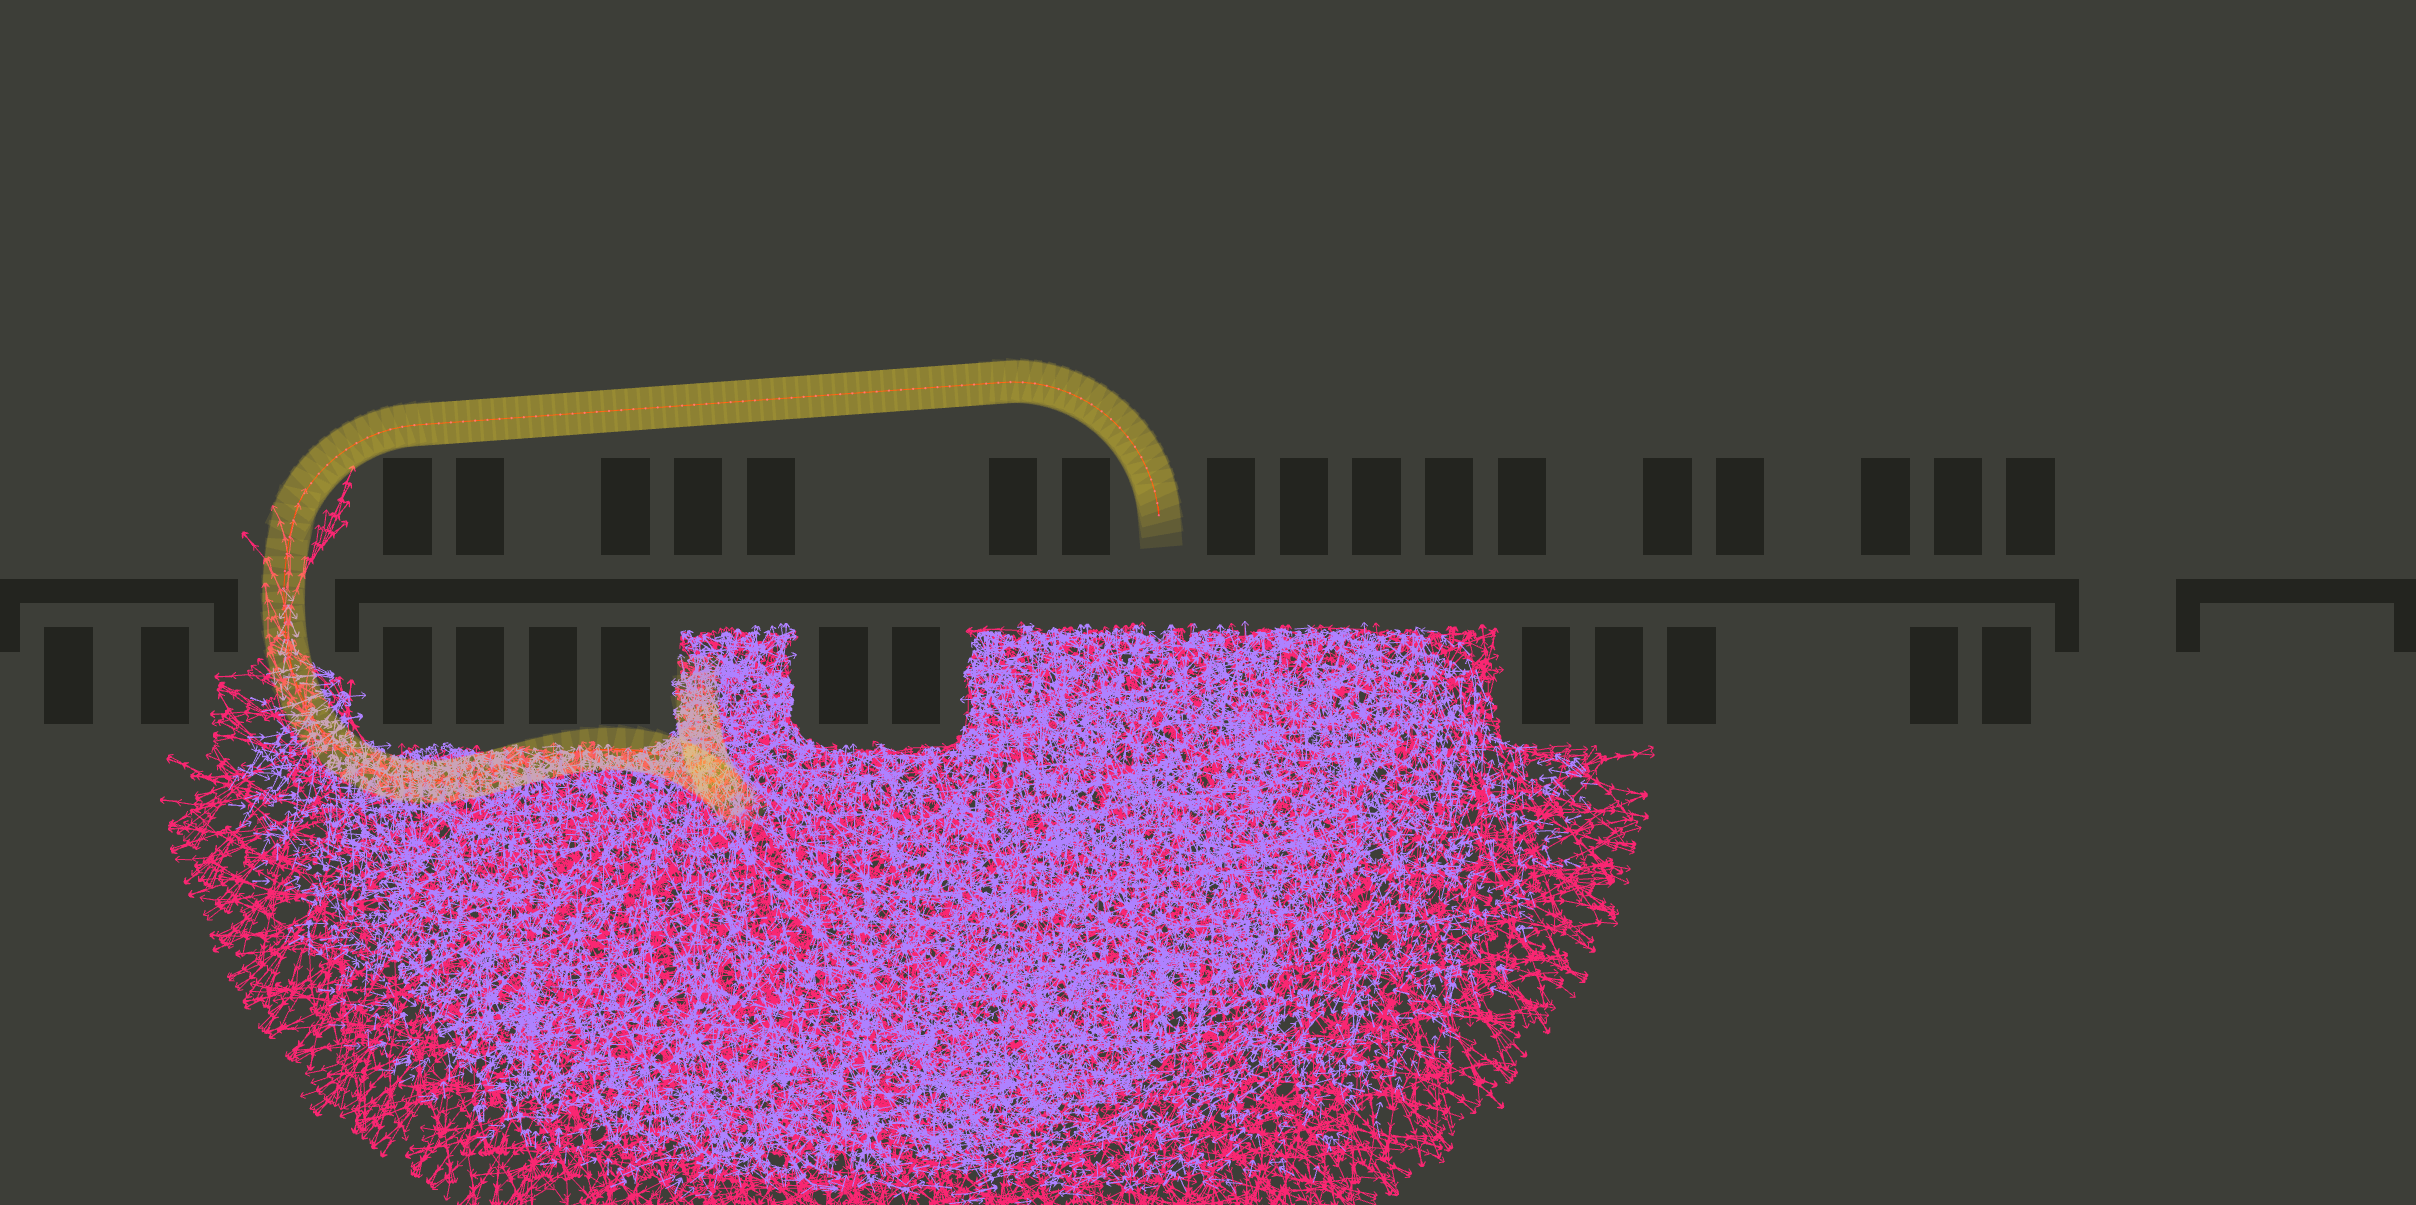
\includegraphics[width=\textwidth]{scenarioParkingReedsShepp.png}
        \caption{Euclidean, 47559 vertices, length x\,m}
    \label{fig:scenarioParkingNo2d}
    \end{subfigure}
    \begin{subfigure}[t]{\textwidth}
    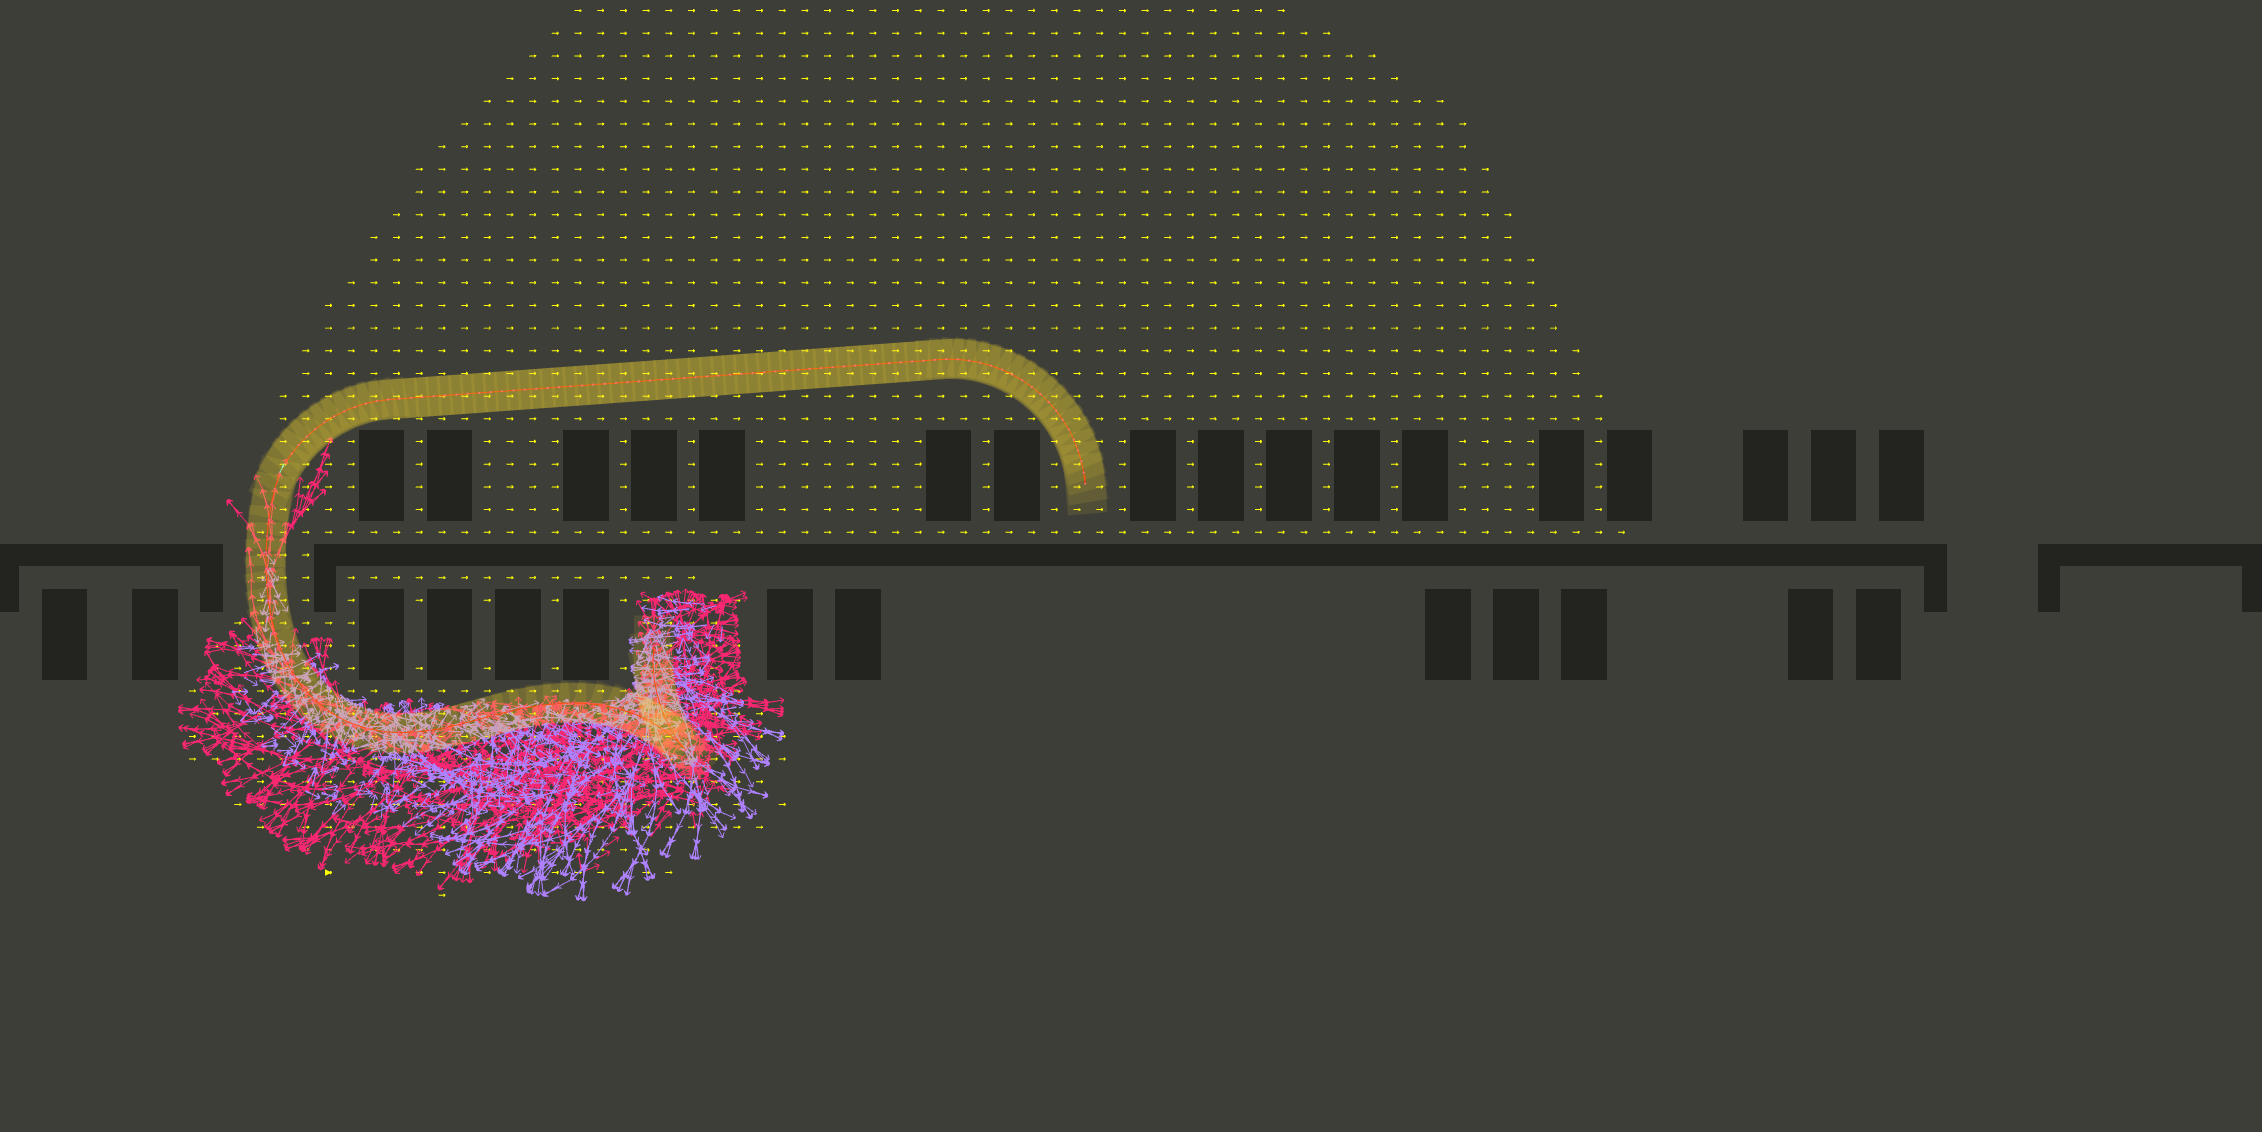
\includegraphics[width=\textwidth]{scenarioParking2d.png}
        \caption{2D A* \& Reeds Shepp, 4767 vertices (1517 vertices), length x\,m}
    \label{fig:scenarioParking2D}
    \end{subfigure}    
    \begin{subfigure}[t]{\textwidth}
    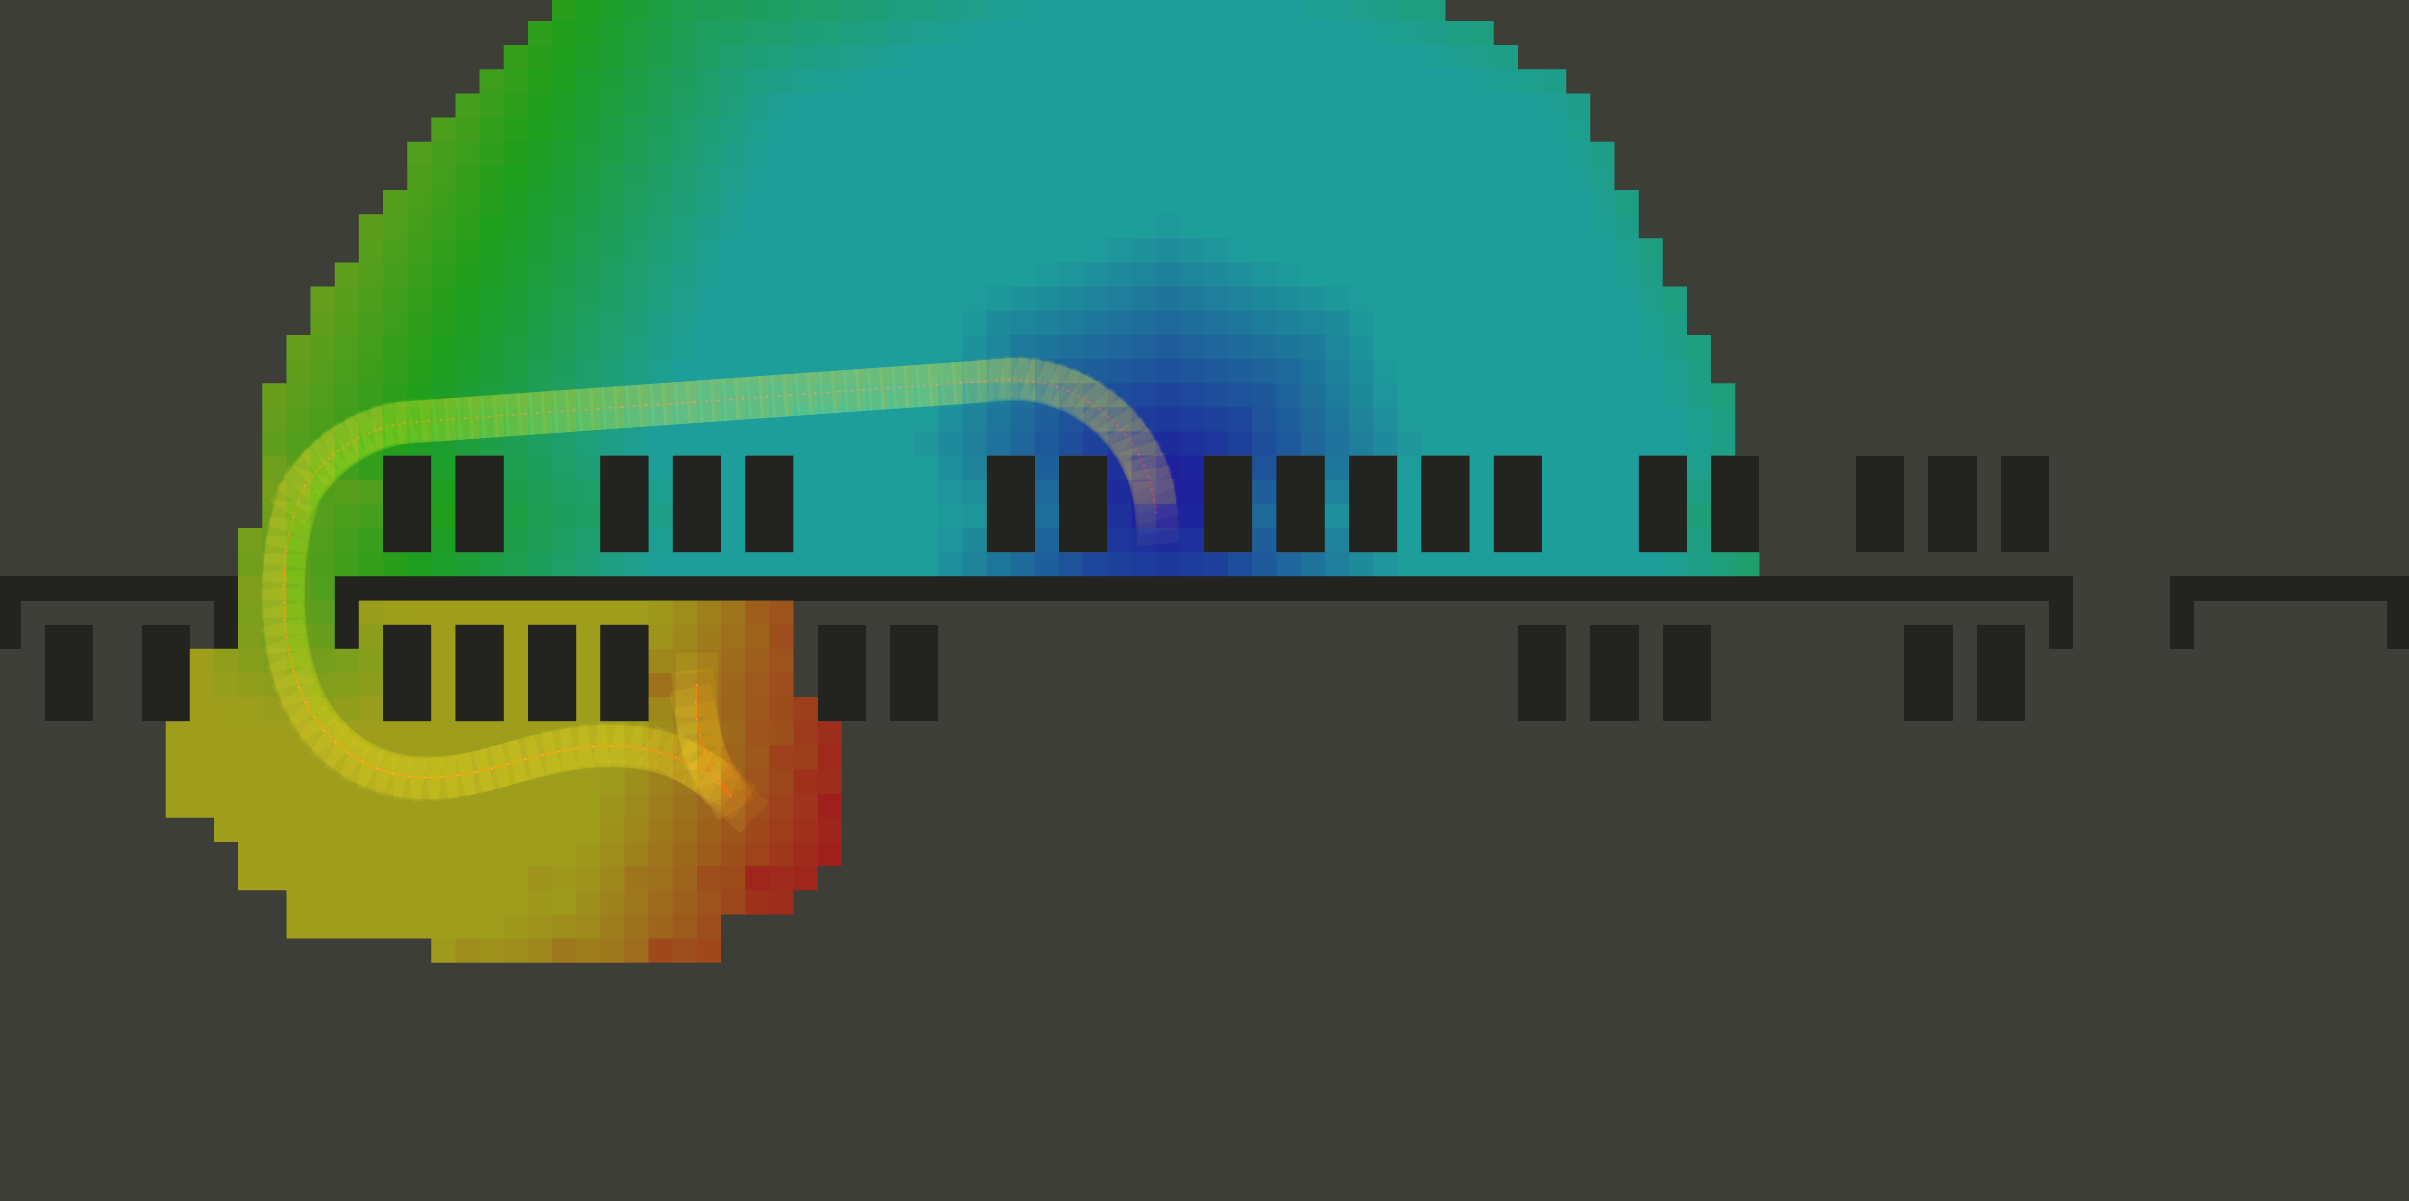
\includegraphics[width=\textwidth]{scenarioParking2dCost.png}
        \caption{2D A* \& Reeds Shepp, 4767 vertices (1517 vertices), length x\,m}
    \label{fig:scenarioParking2dCost}
    \end{subfigure}
    \caption{The parking structure scenario}
    \label{fig:scenarioParking}
\end{figure}

\subsection{Obstacles}

\begin{figure}[h]
    \centering
    \begin{subfigure}[t]{\textwidth}
        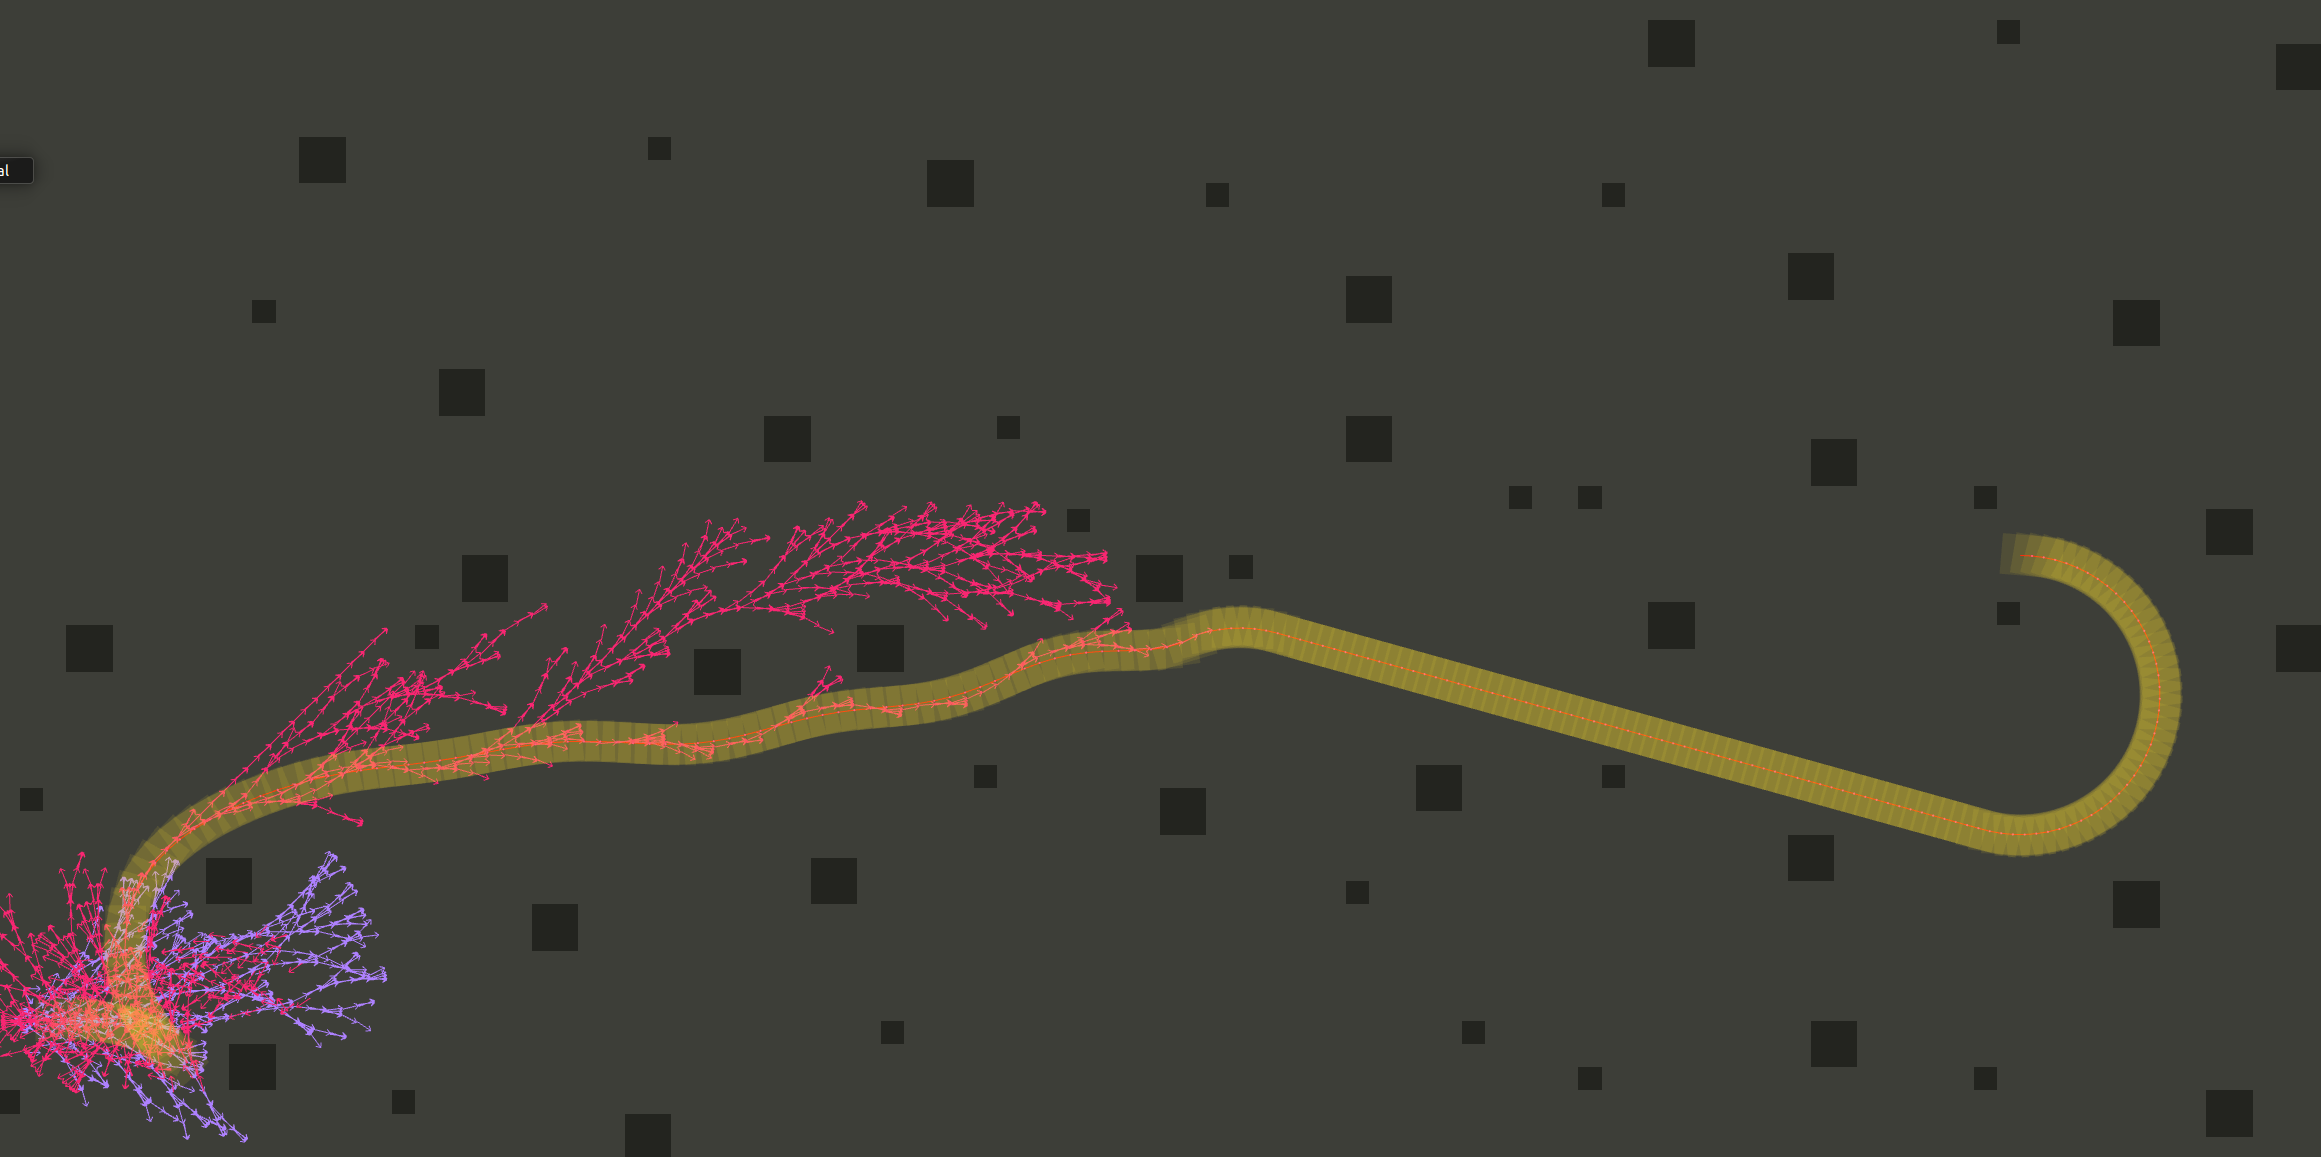
\includegraphics[width=\textwidth]{scenarioObstacles2d.png}
        \caption{2D A*, 2685 vertices, length 116.882\,m}
        \label{fig:scenarioObstacles2d}
    \end{subfigure}
    \begin{subfigure}[t]{\textwidth}
        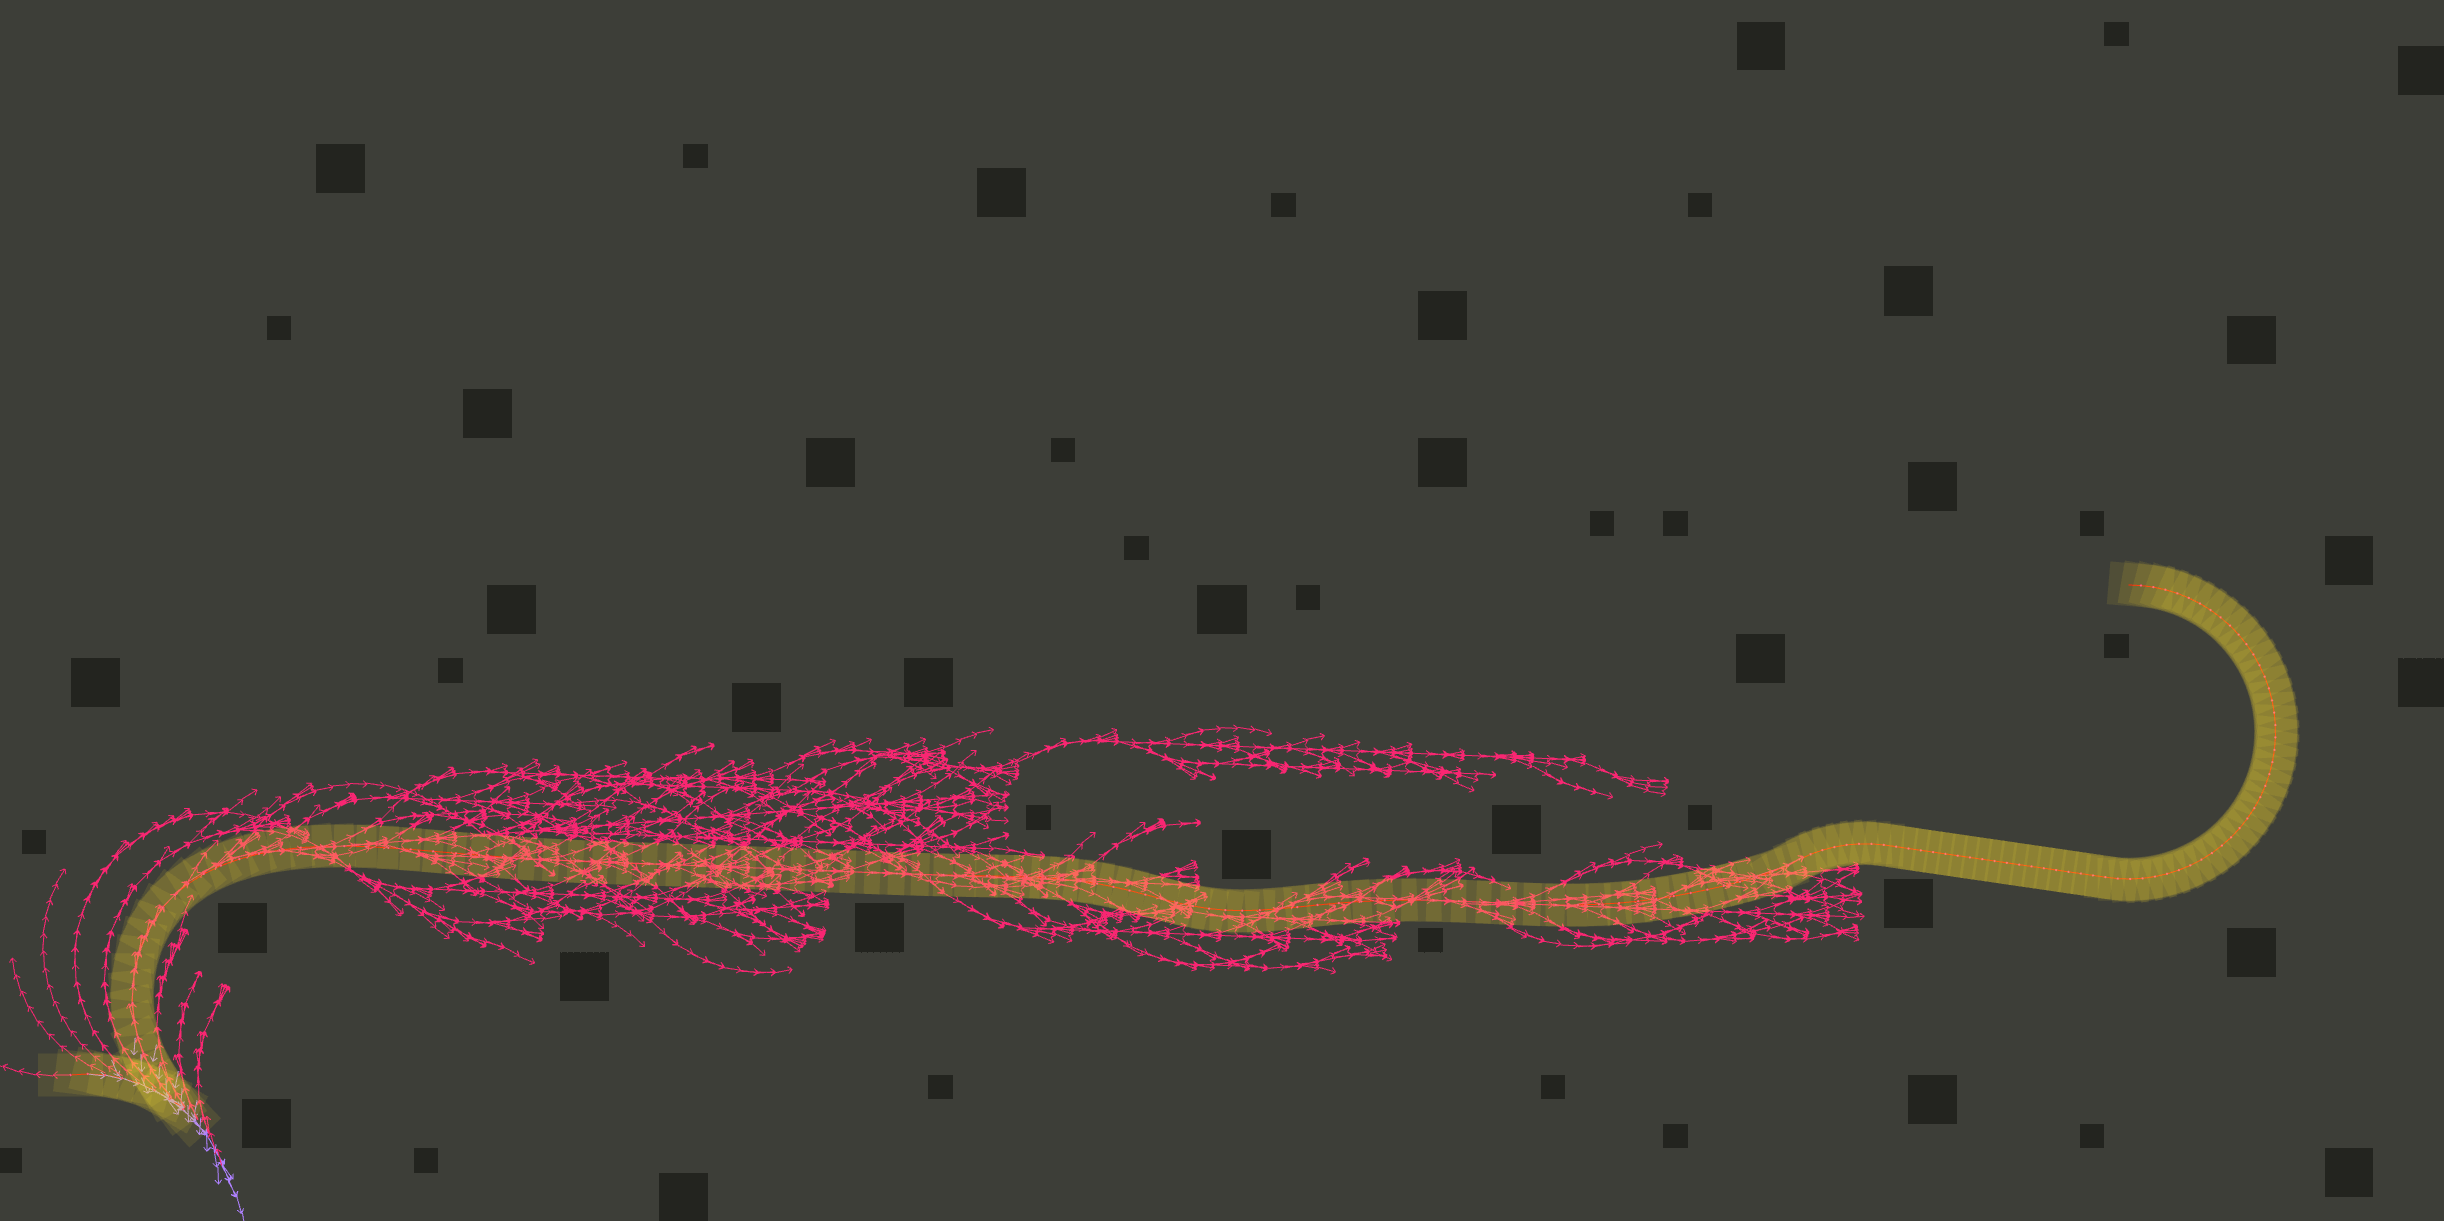
\includegraphics[width=\textwidth]{scenarioObstacles2dDubins.png}
        \caption{2D A* \& Dubins, 3486 vertices, length 114.961\,m}
        \label{fig:scenarioObstacles2dDubins}
    \end{subfigure}    
    \begin{subfigure}[t]{\textwidth}
        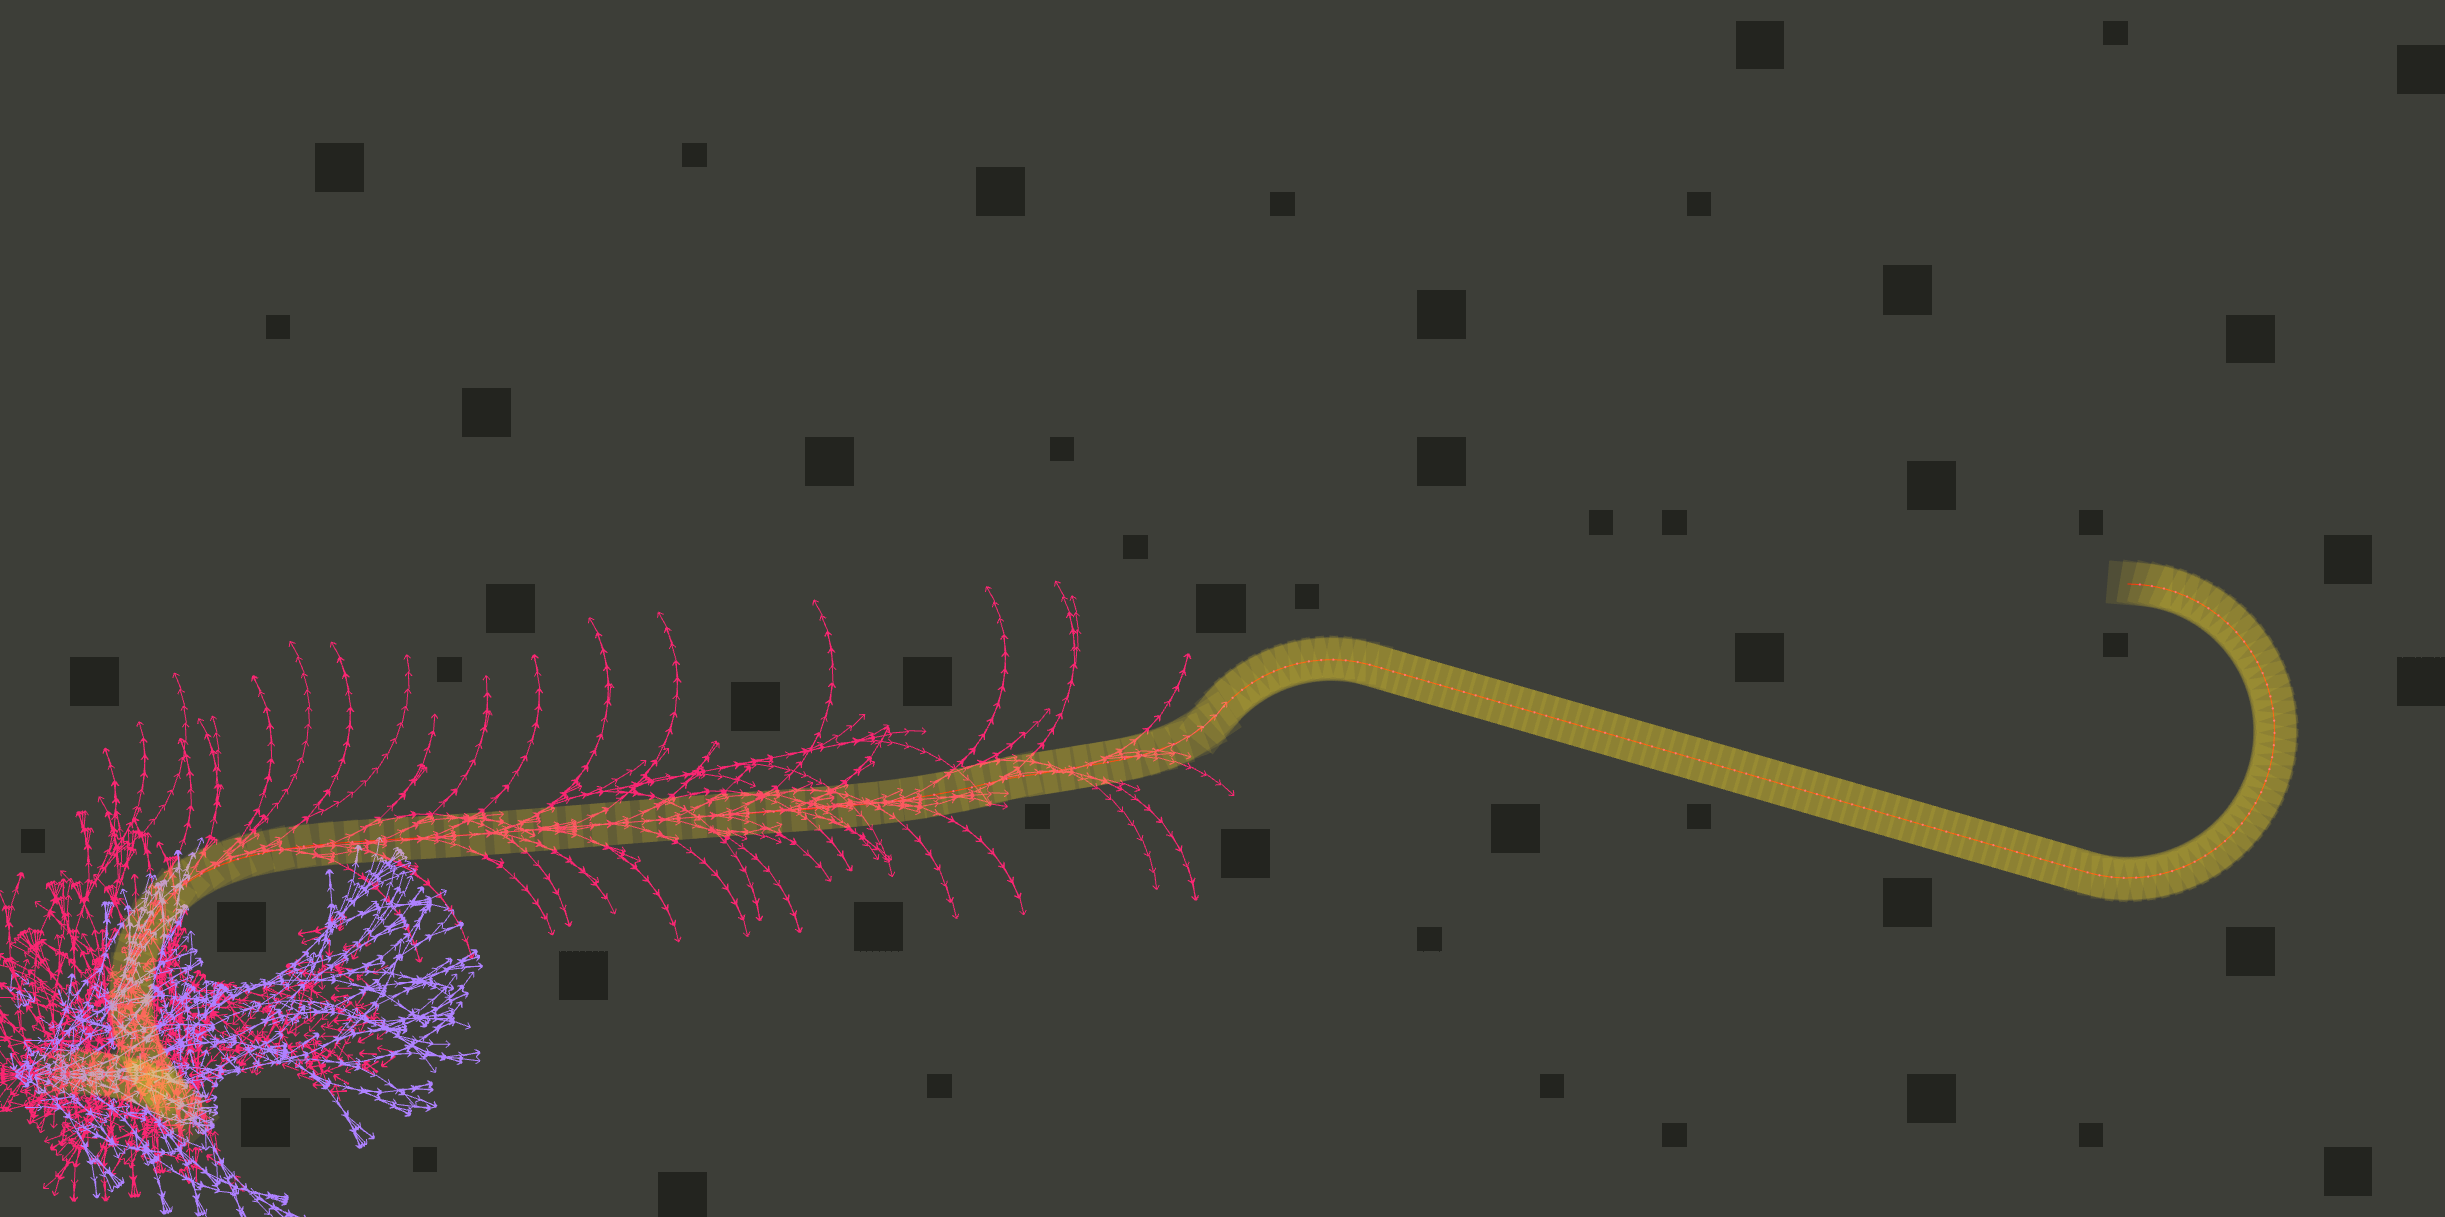
\includegraphics[width=\textwidth]{scenarioObstacles2dReedsShepp.png}
        \caption{2D A* \& Reeds Shepp, 4316 vertices, length 116.647\,m}
        \label{fig:scenarioObstacles2dReedsShepp}
    \end{subfigure}
%    \begin{subfigure}[t]{\textwidth}
%        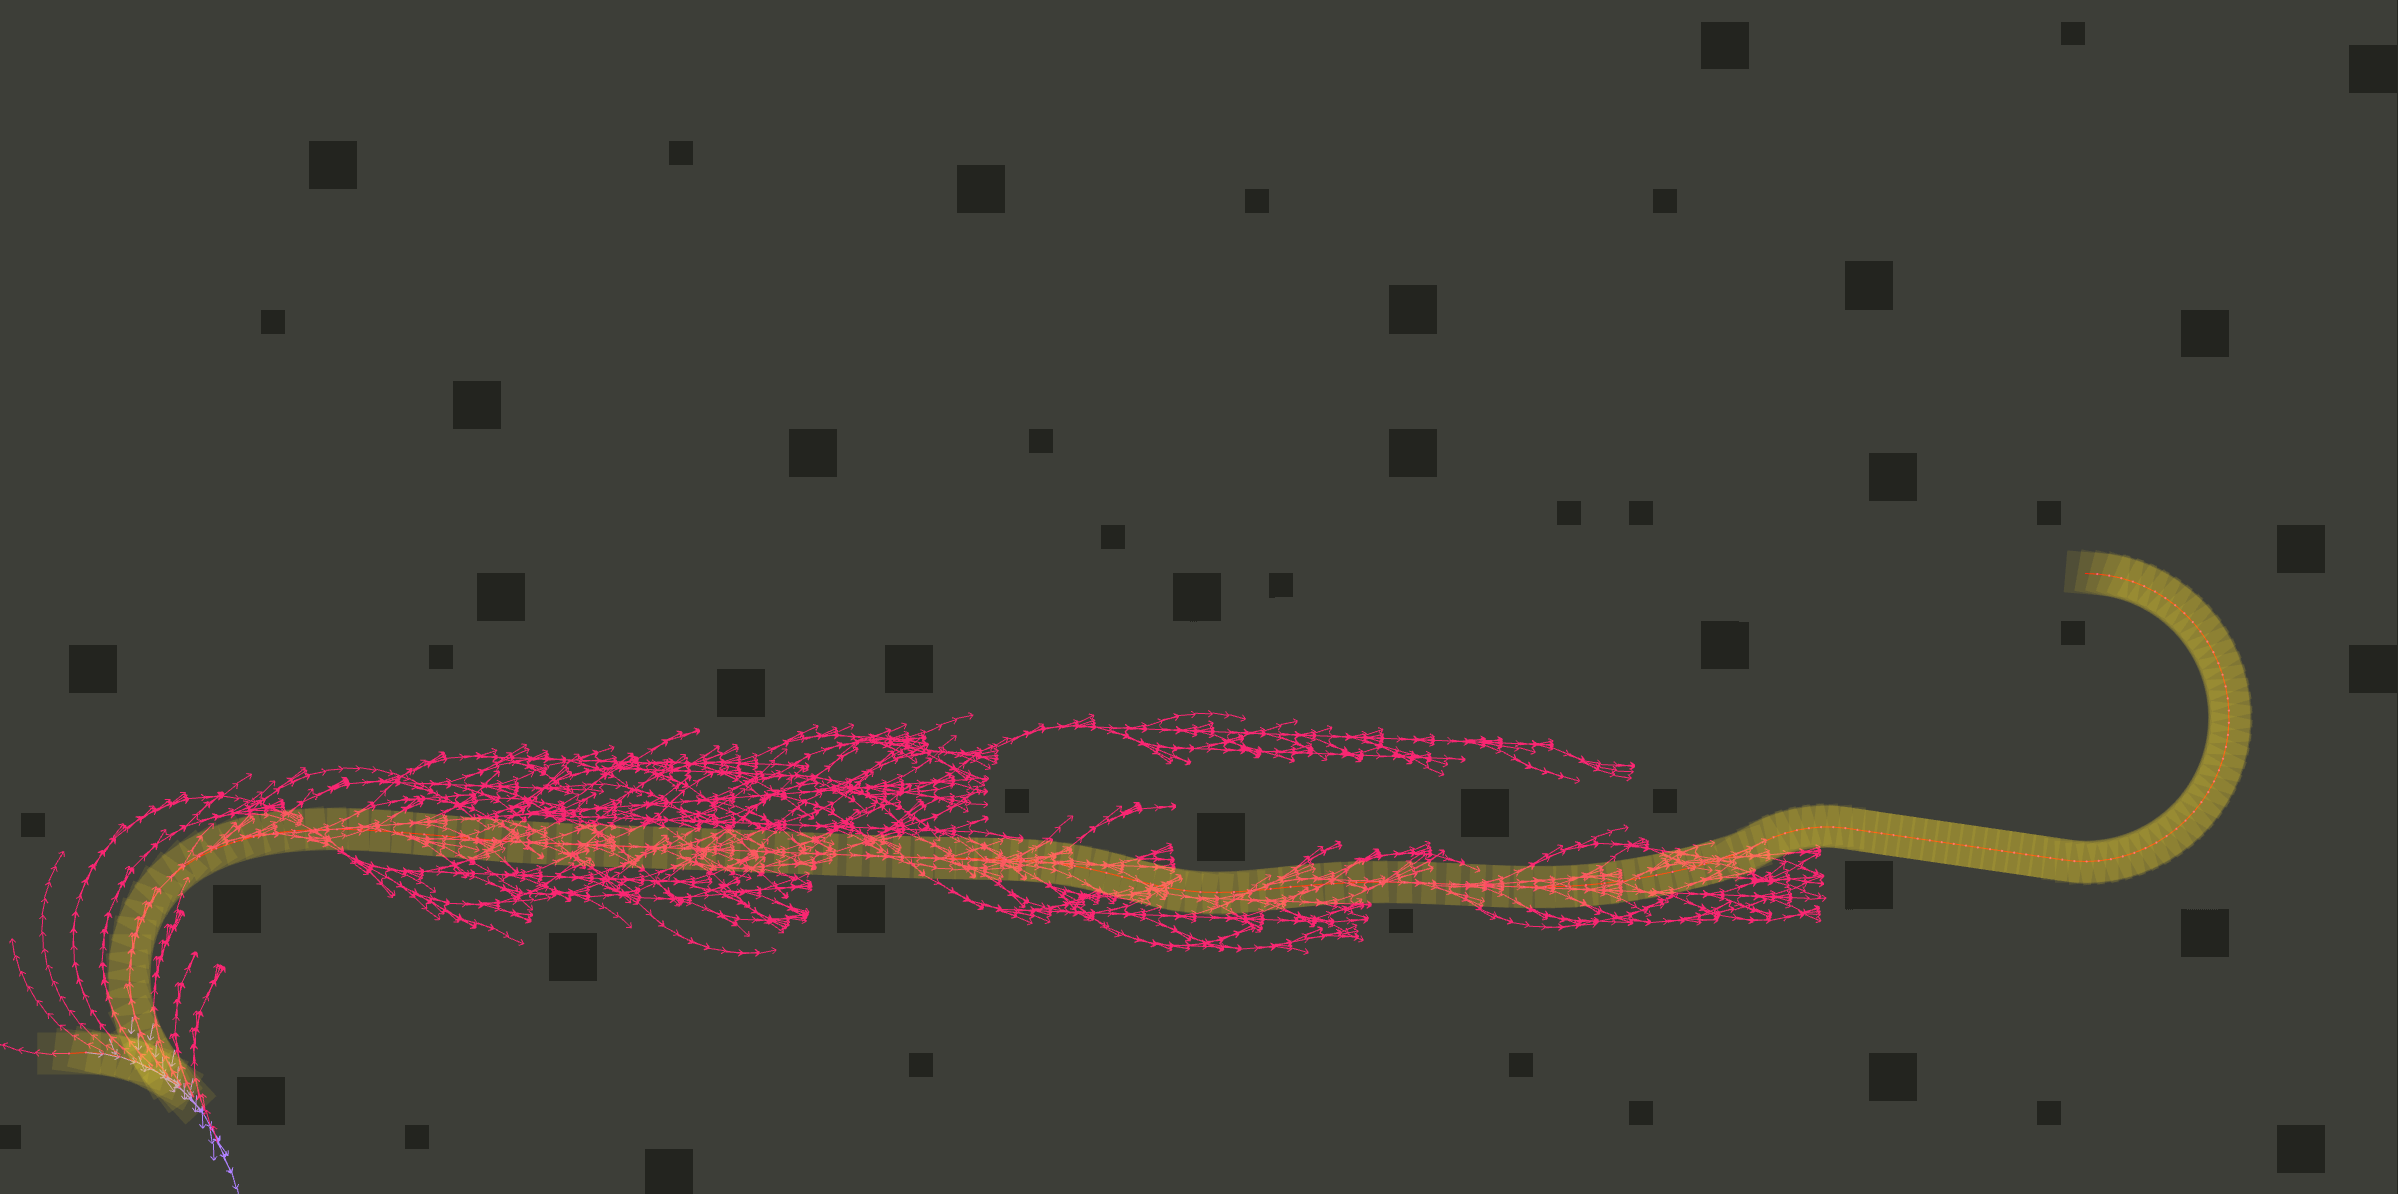
\includegraphics[width=\textwidth]{scenarioObstaclesDubins.png}
%        \caption{Dubins, 3486 vertices, length 114.961\,m}
%        \label{fig:scenarioObstaclesDubins}
%    \end{subfigure}
%    \begin{subfigure}[t]{\textwidth}
%        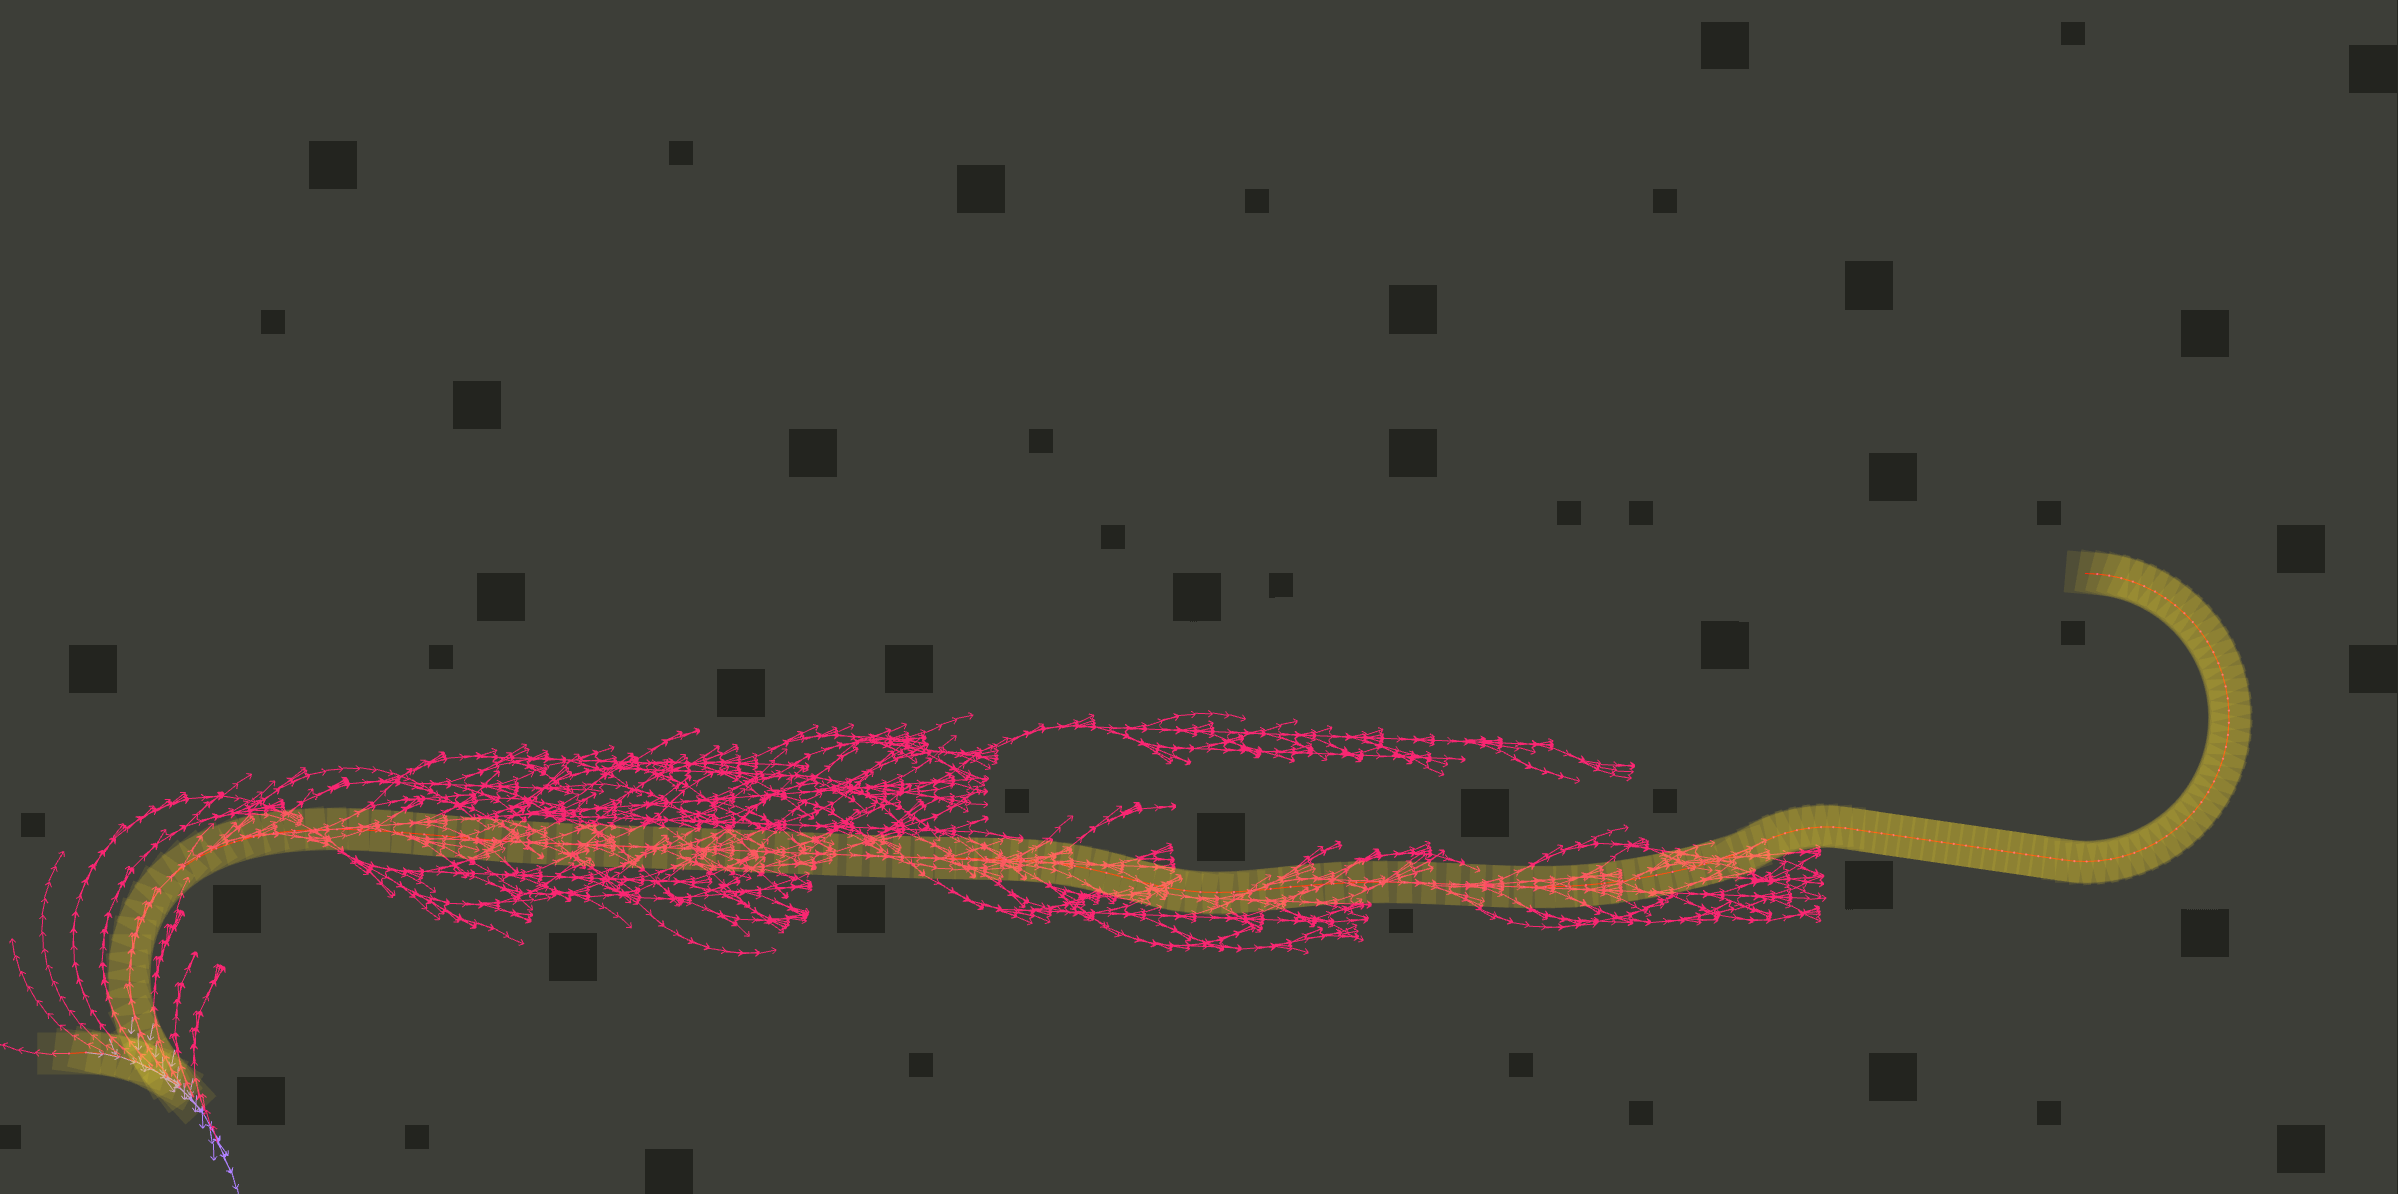
\includegraphics[width=\textwidth]{scenarioObstaclesDubins.png}
%        \caption{Reeds Shepp, 3486 vertices, length 116.141\,m}
%        \label{fig:scenarioObstaclesDubins}
%    \end{subfigure}
    \caption{The obstacle scenario}
    \label{fig:scenarioObstacle}
\end{figure}

\subsection{Wall}

\begin{figure}[h]
    \centering
    \begin{subfigure}[t]{\textwidth}
        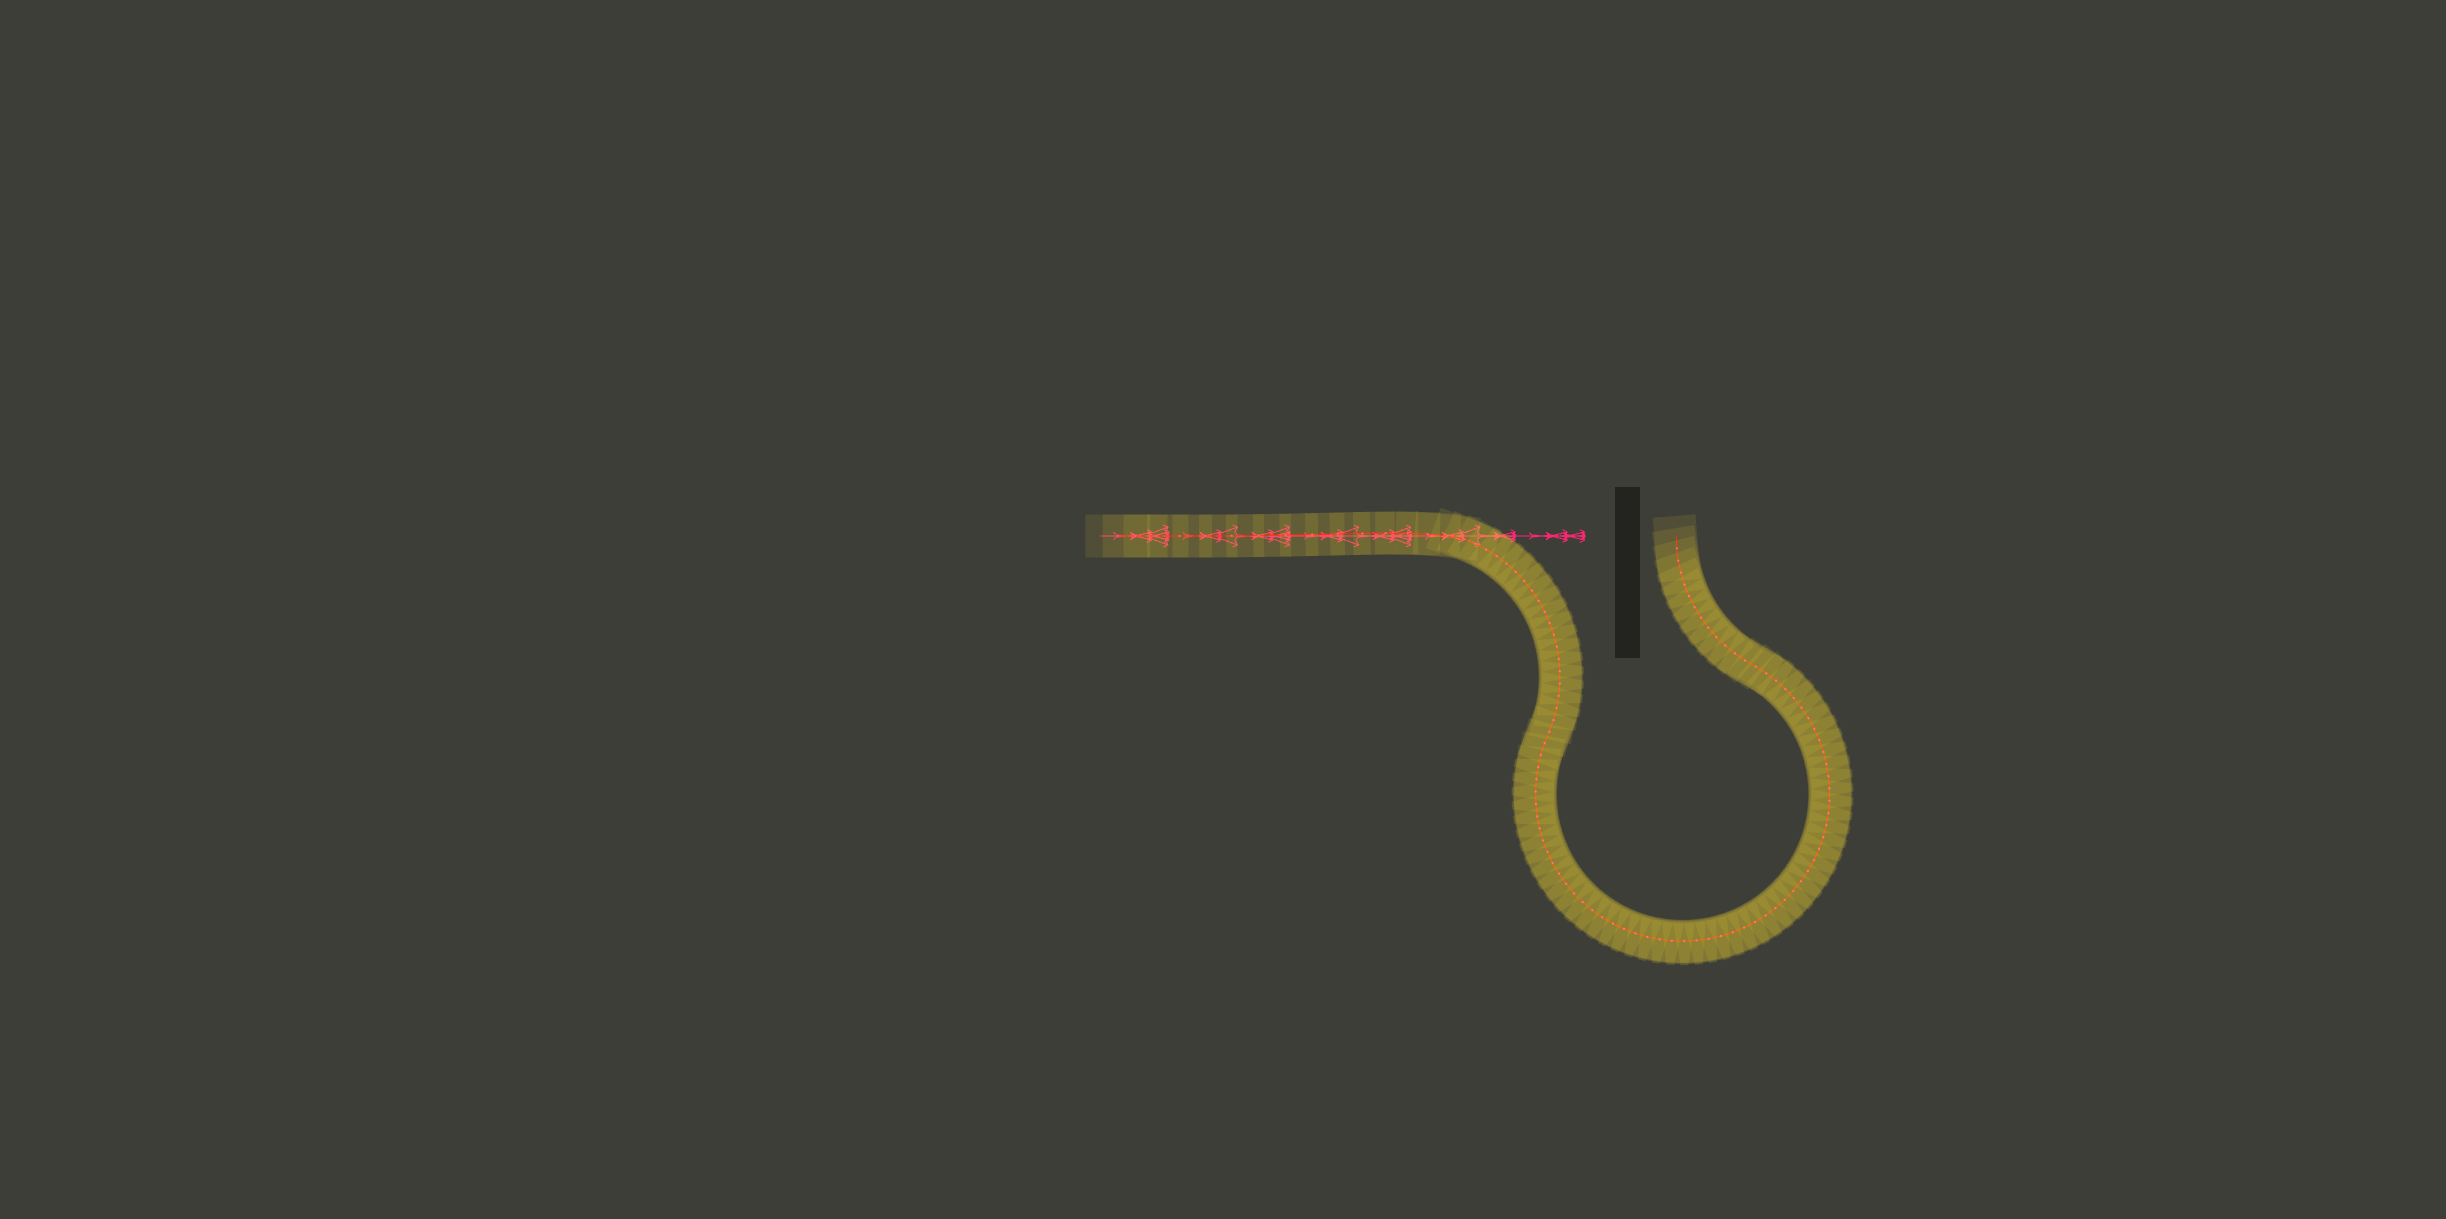
\includegraphics[width=\textwidth]{scenarioWall.png}
        \caption{Euclidean, 237 vertices, length 58.224,m}
        \label{fig:scenarioWall}
    \end{subfigure}
    \begin{subfigure}[t]{\textwidth}
        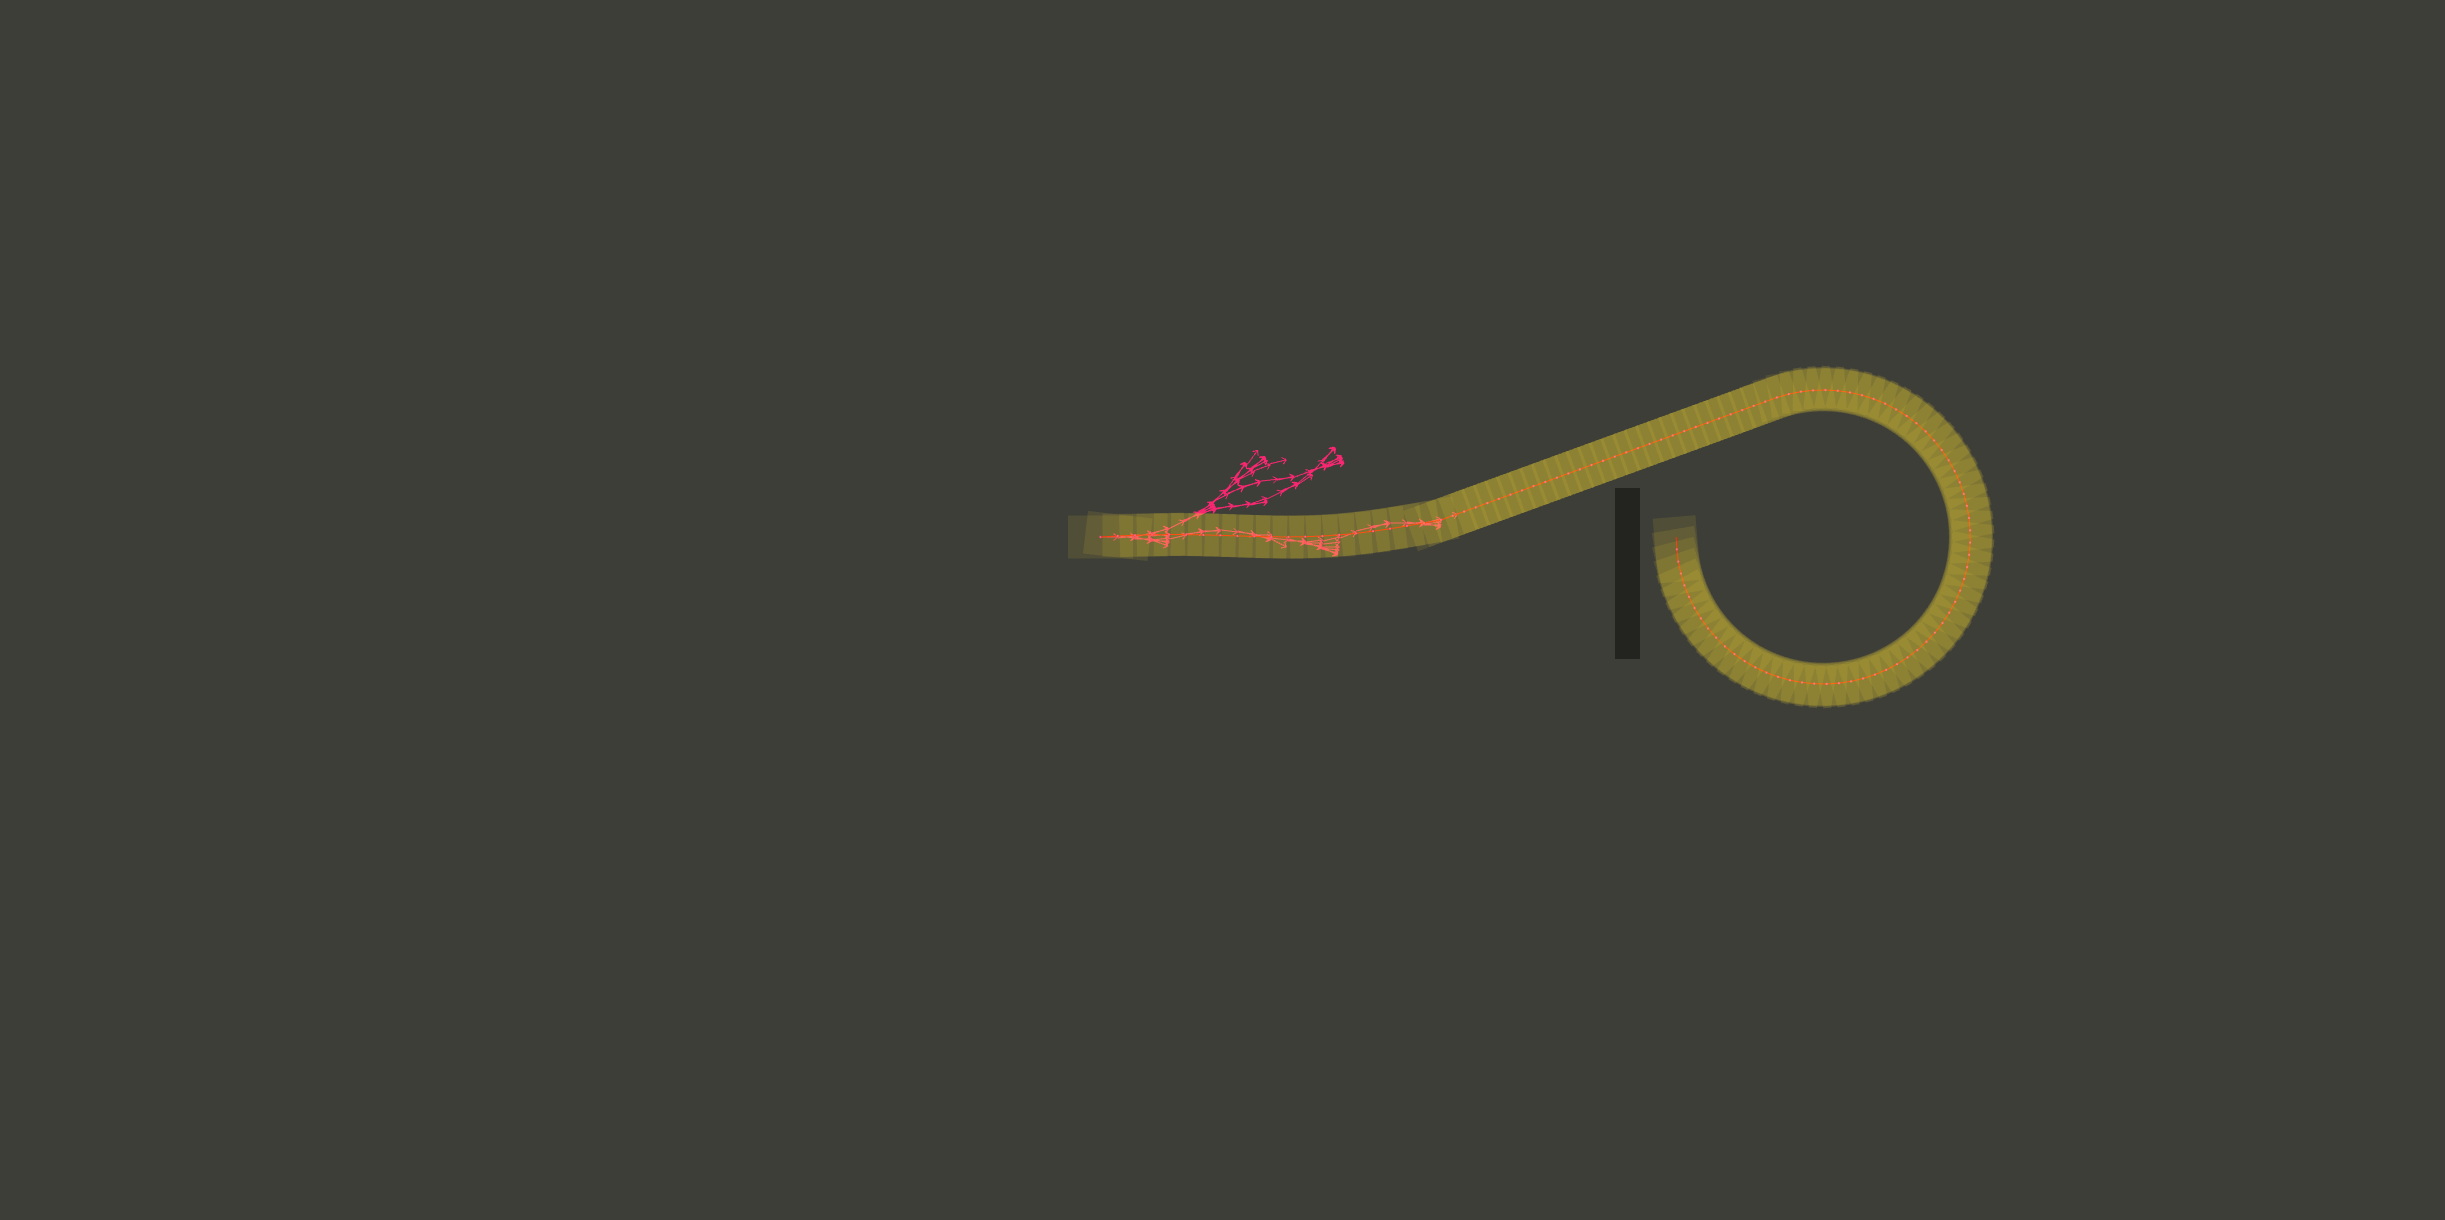
\includegraphics[width=\textwidth]{scenarioWall2d.png}
        \caption{2D A*, 129 vertices, length 58.914\,m}
        \label{fig:scenarioWall2d}
    \end{subfigure}    
    \begin{subfigure}[t]{\textwidth}
        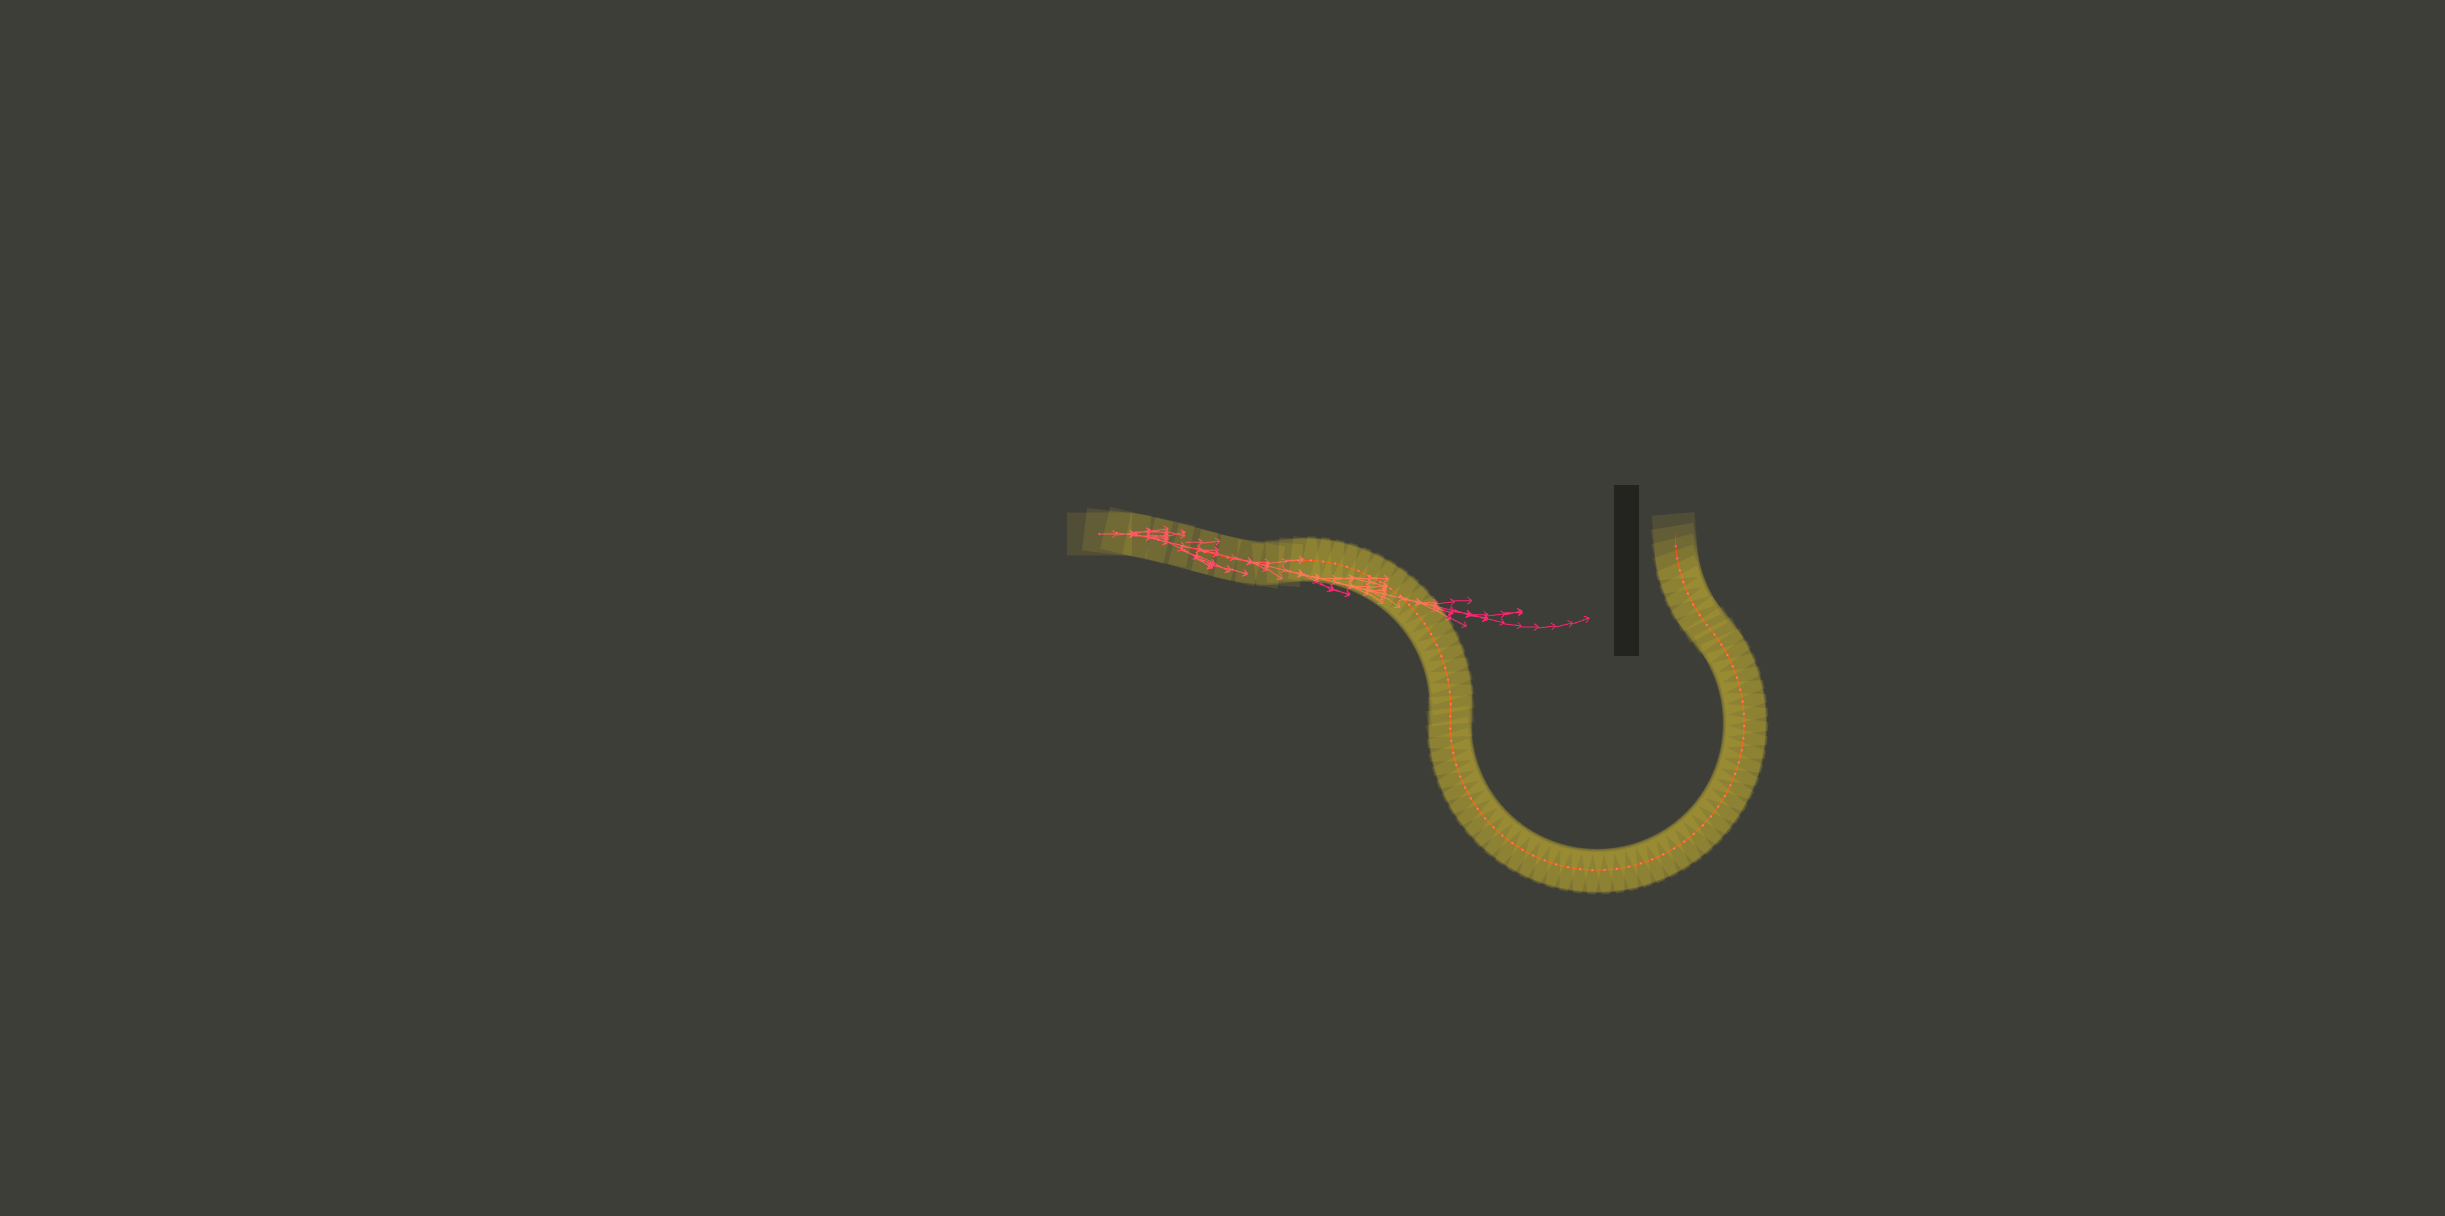
\includegraphics[width=\textwidth]{scenarioWallReedsShepp.png}
        \caption{Reeds Shepp, 124 vertices, length 45.780\,m}
        \label{fig:scenarioWallReedsShepp}
    \end{subfigure}
    \caption{The wall scenario}
    \label{fig:scenarioWall}
\end{figure}

\subsection{Dead End}

\begin{figure}[h]
    \centering
    \begin{subfigure}[t]{\textwidth}
        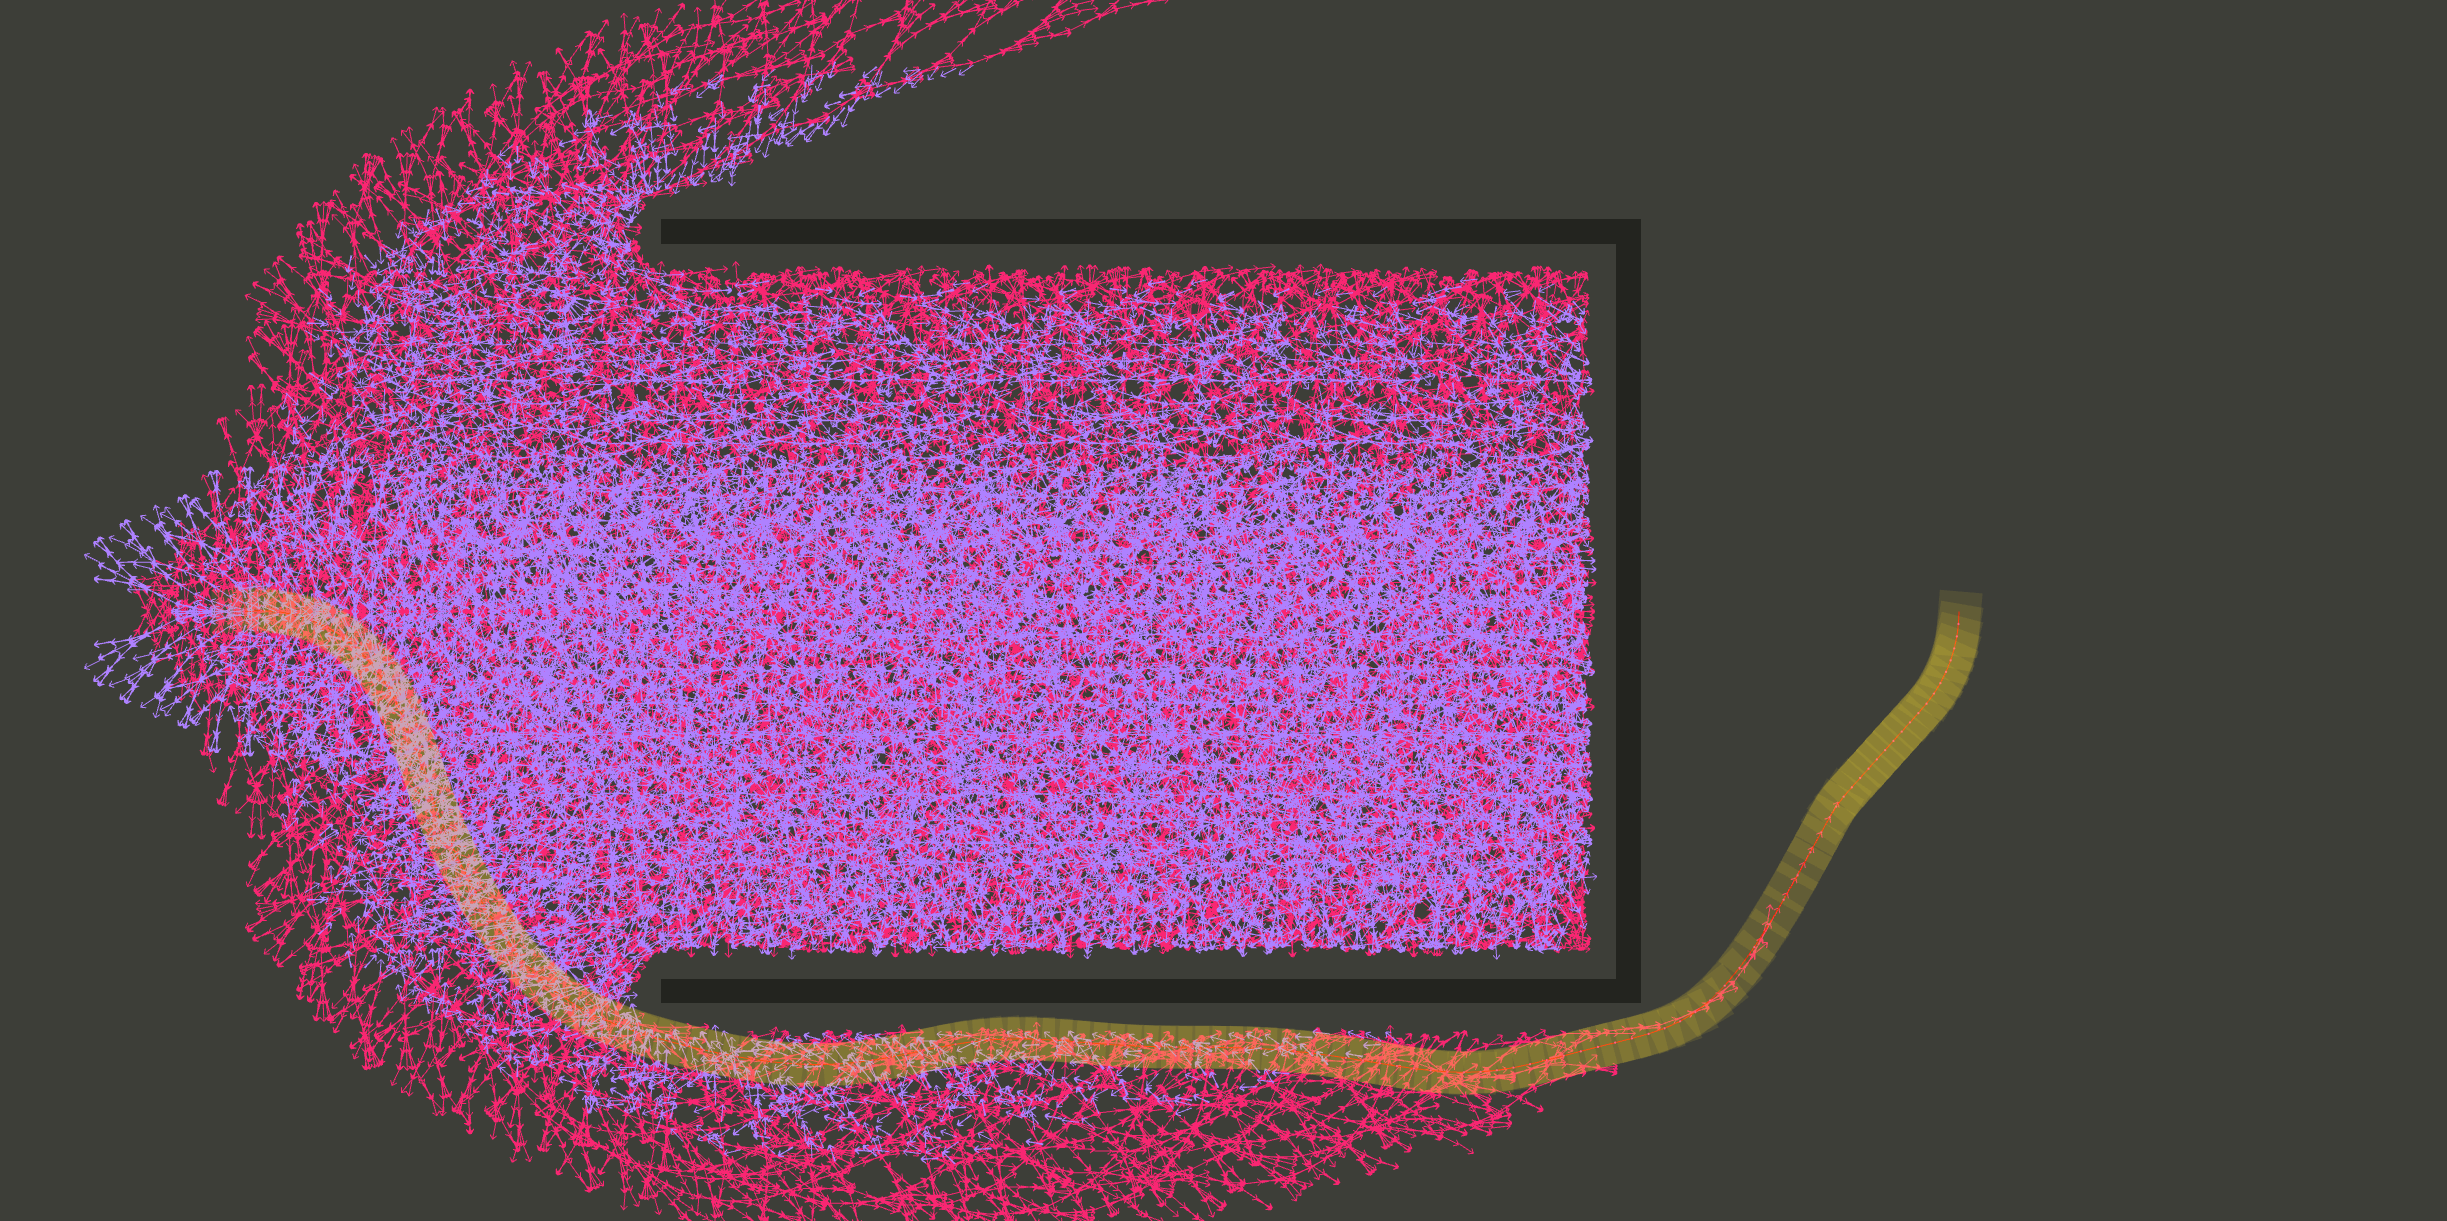
\includegraphics[width=\textwidth]{scenarioDeadEnd.png}
        \caption{Euclidean, 72014 vertices, length 90.0001\,m}
        \label{fig:scenarioDeadEnd}
    \end{subfigure}
    \begin{subfigure}[t]{\textwidth}
        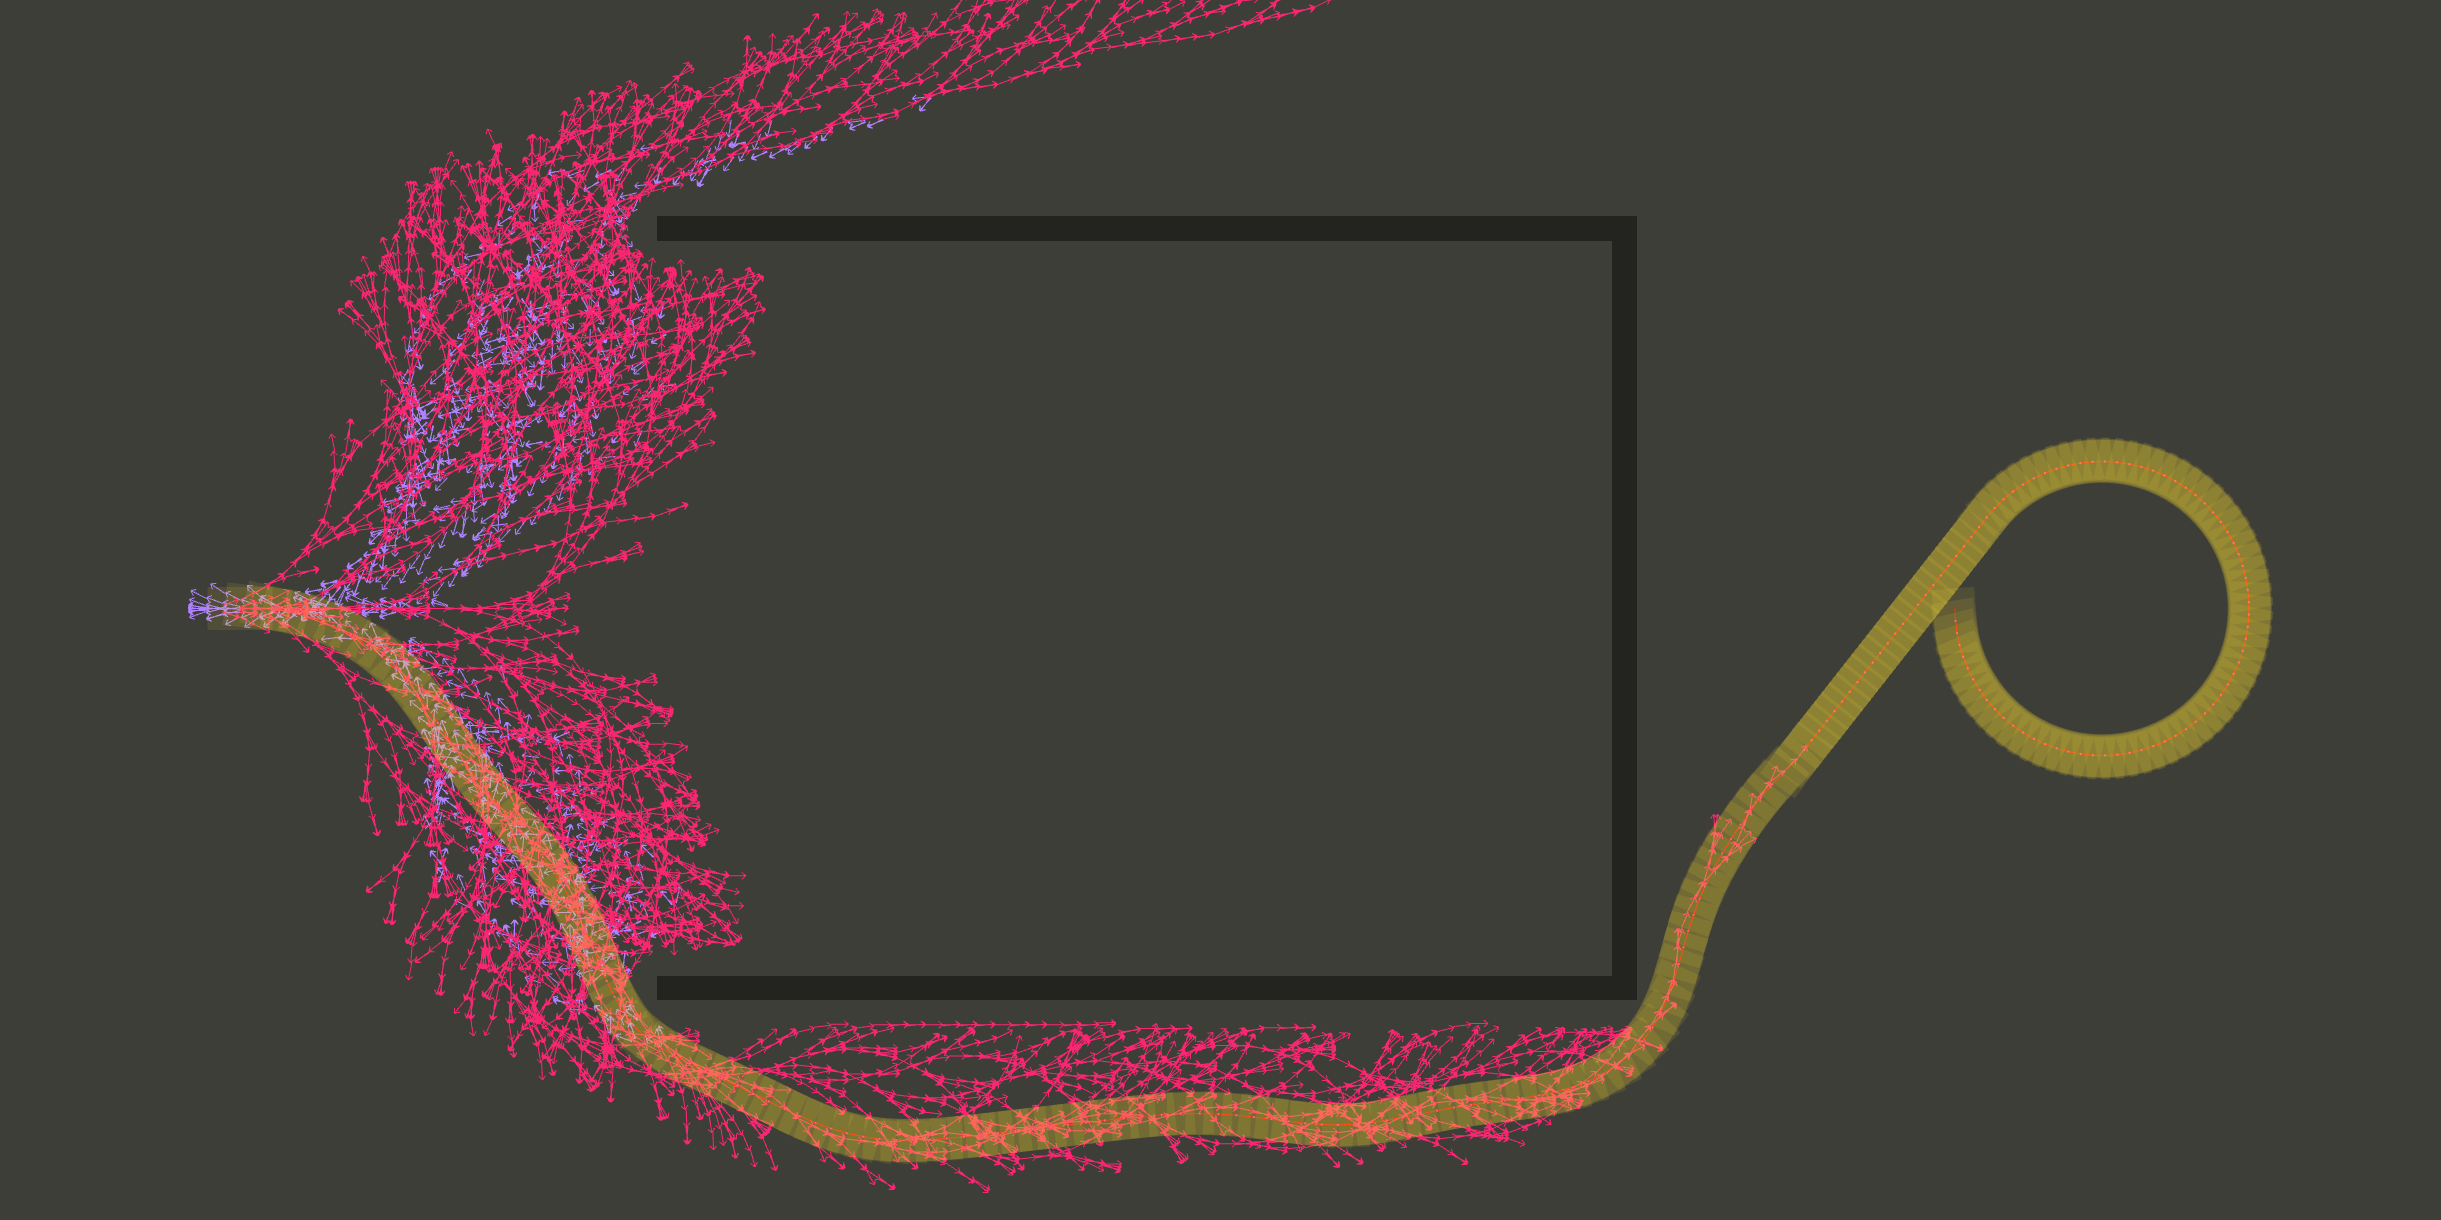
\includegraphics[width=\textwidth]{scenarioDeadEnd2d.png}
        \caption{2D A*, 8871 vertices, length 128.197\,m}
        \label{fig:scenarioDeadEnd2d}
    \end{subfigure}    
    \begin{subfigure}[t]{\textwidth}
        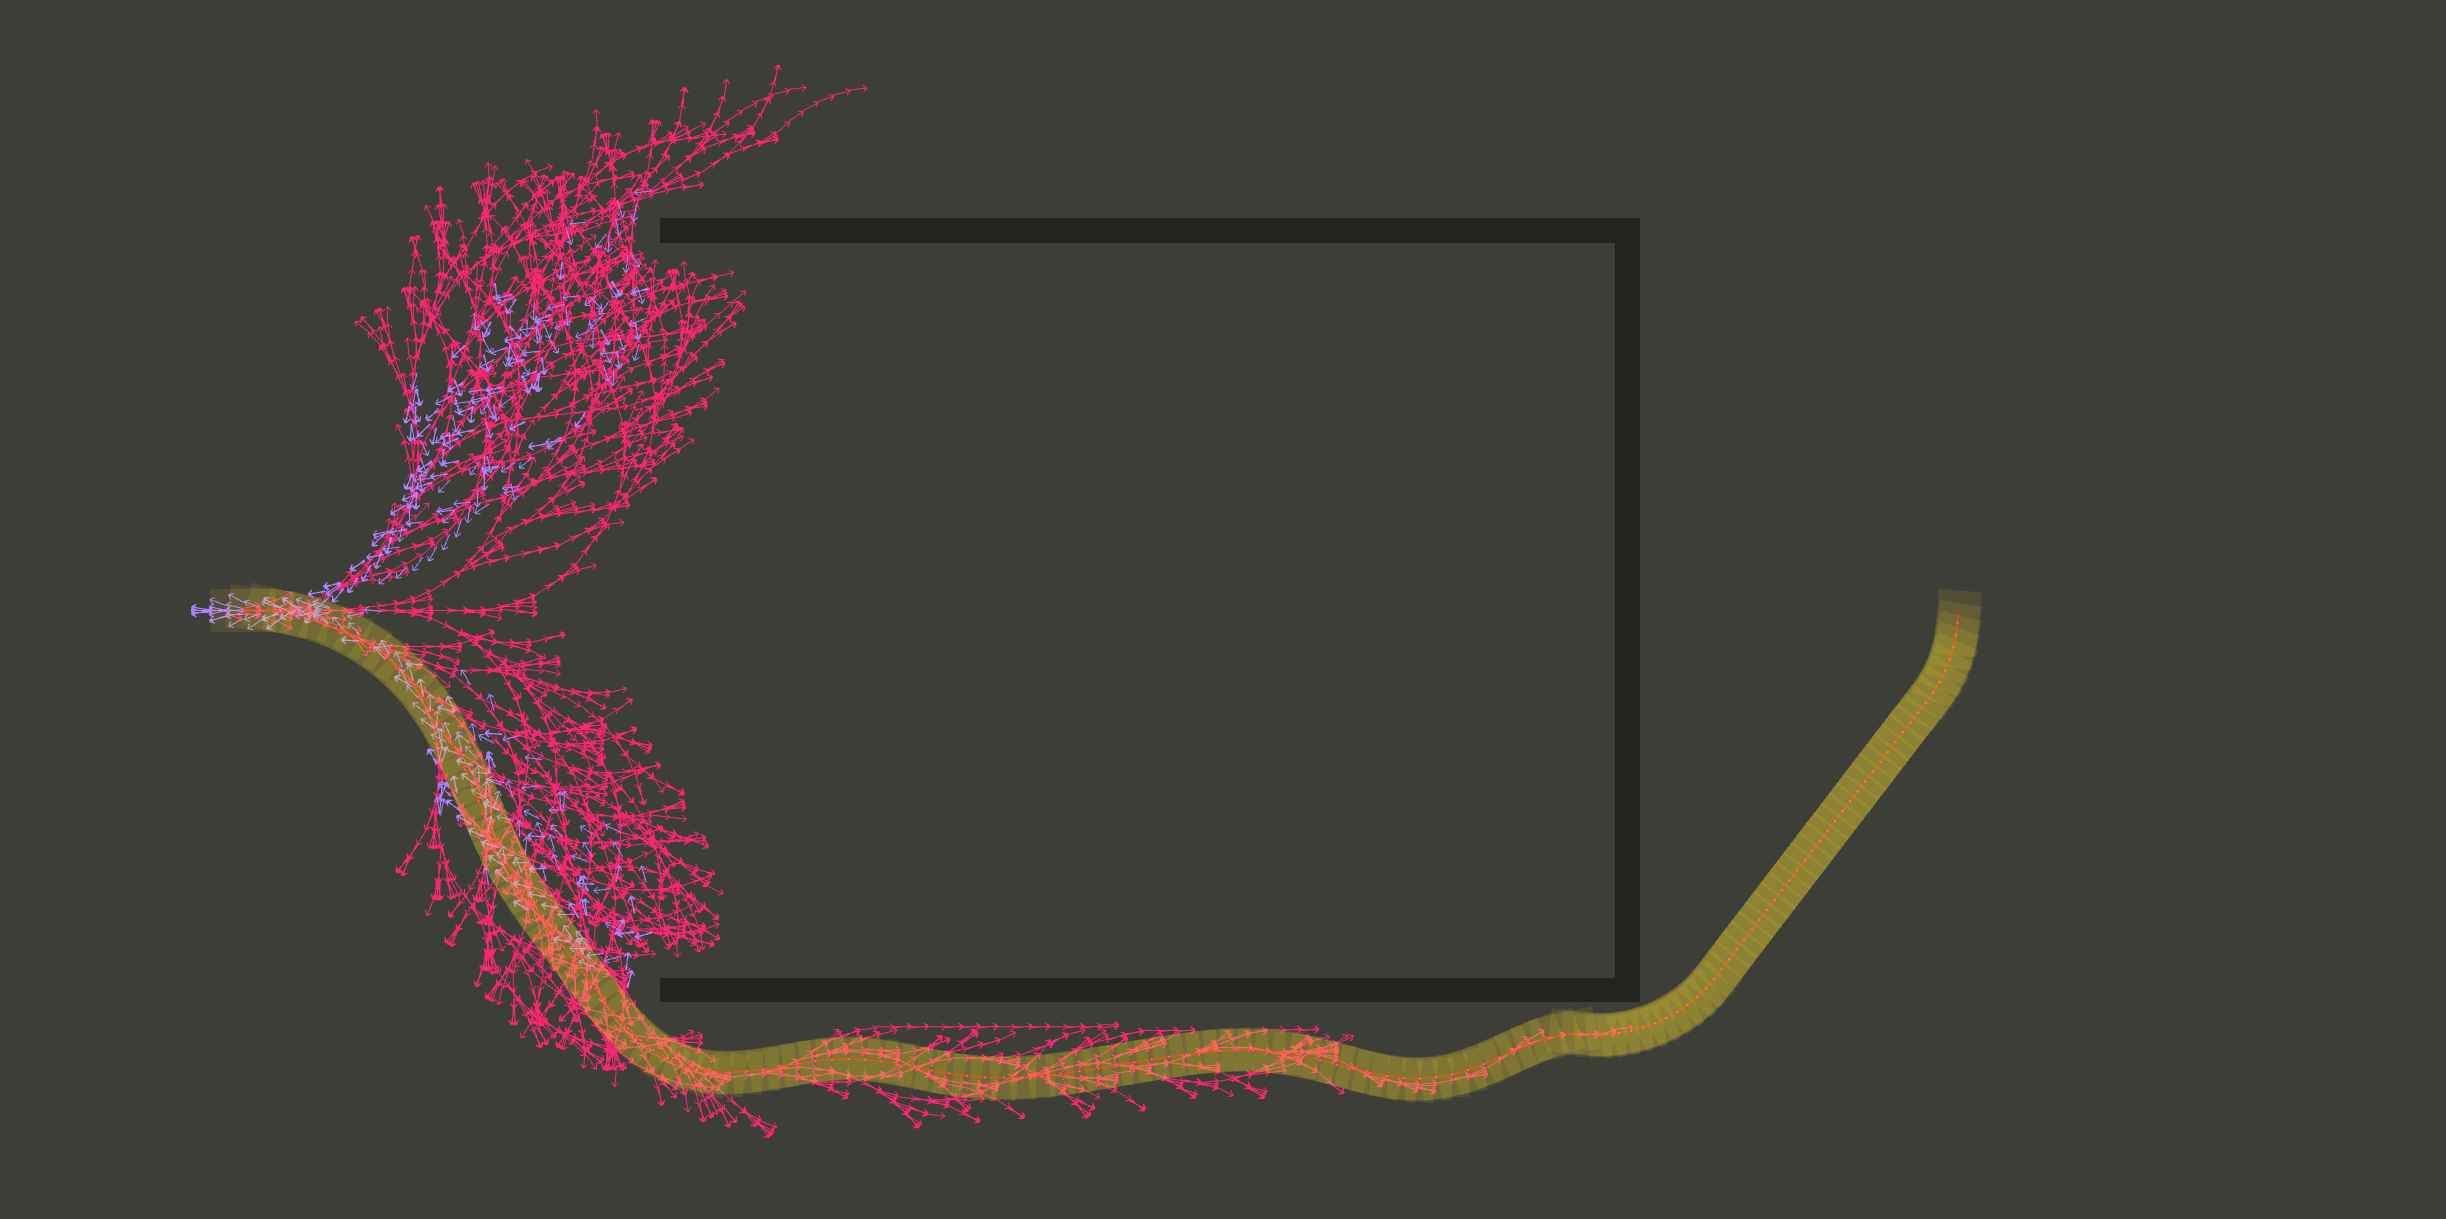
\includegraphics[width=\textwidth]{scenarioDeadEnd2dReedsShepp.png}
        \caption{2D A* \& Reeds Shepp, 8691 vertices, length 90.9778\,m}
        \label{fig:scenarioDeadEnd2dReedsShepp}
    \end{subfigure}
%    \begin{subfigure}[t]{\textwidth}
%        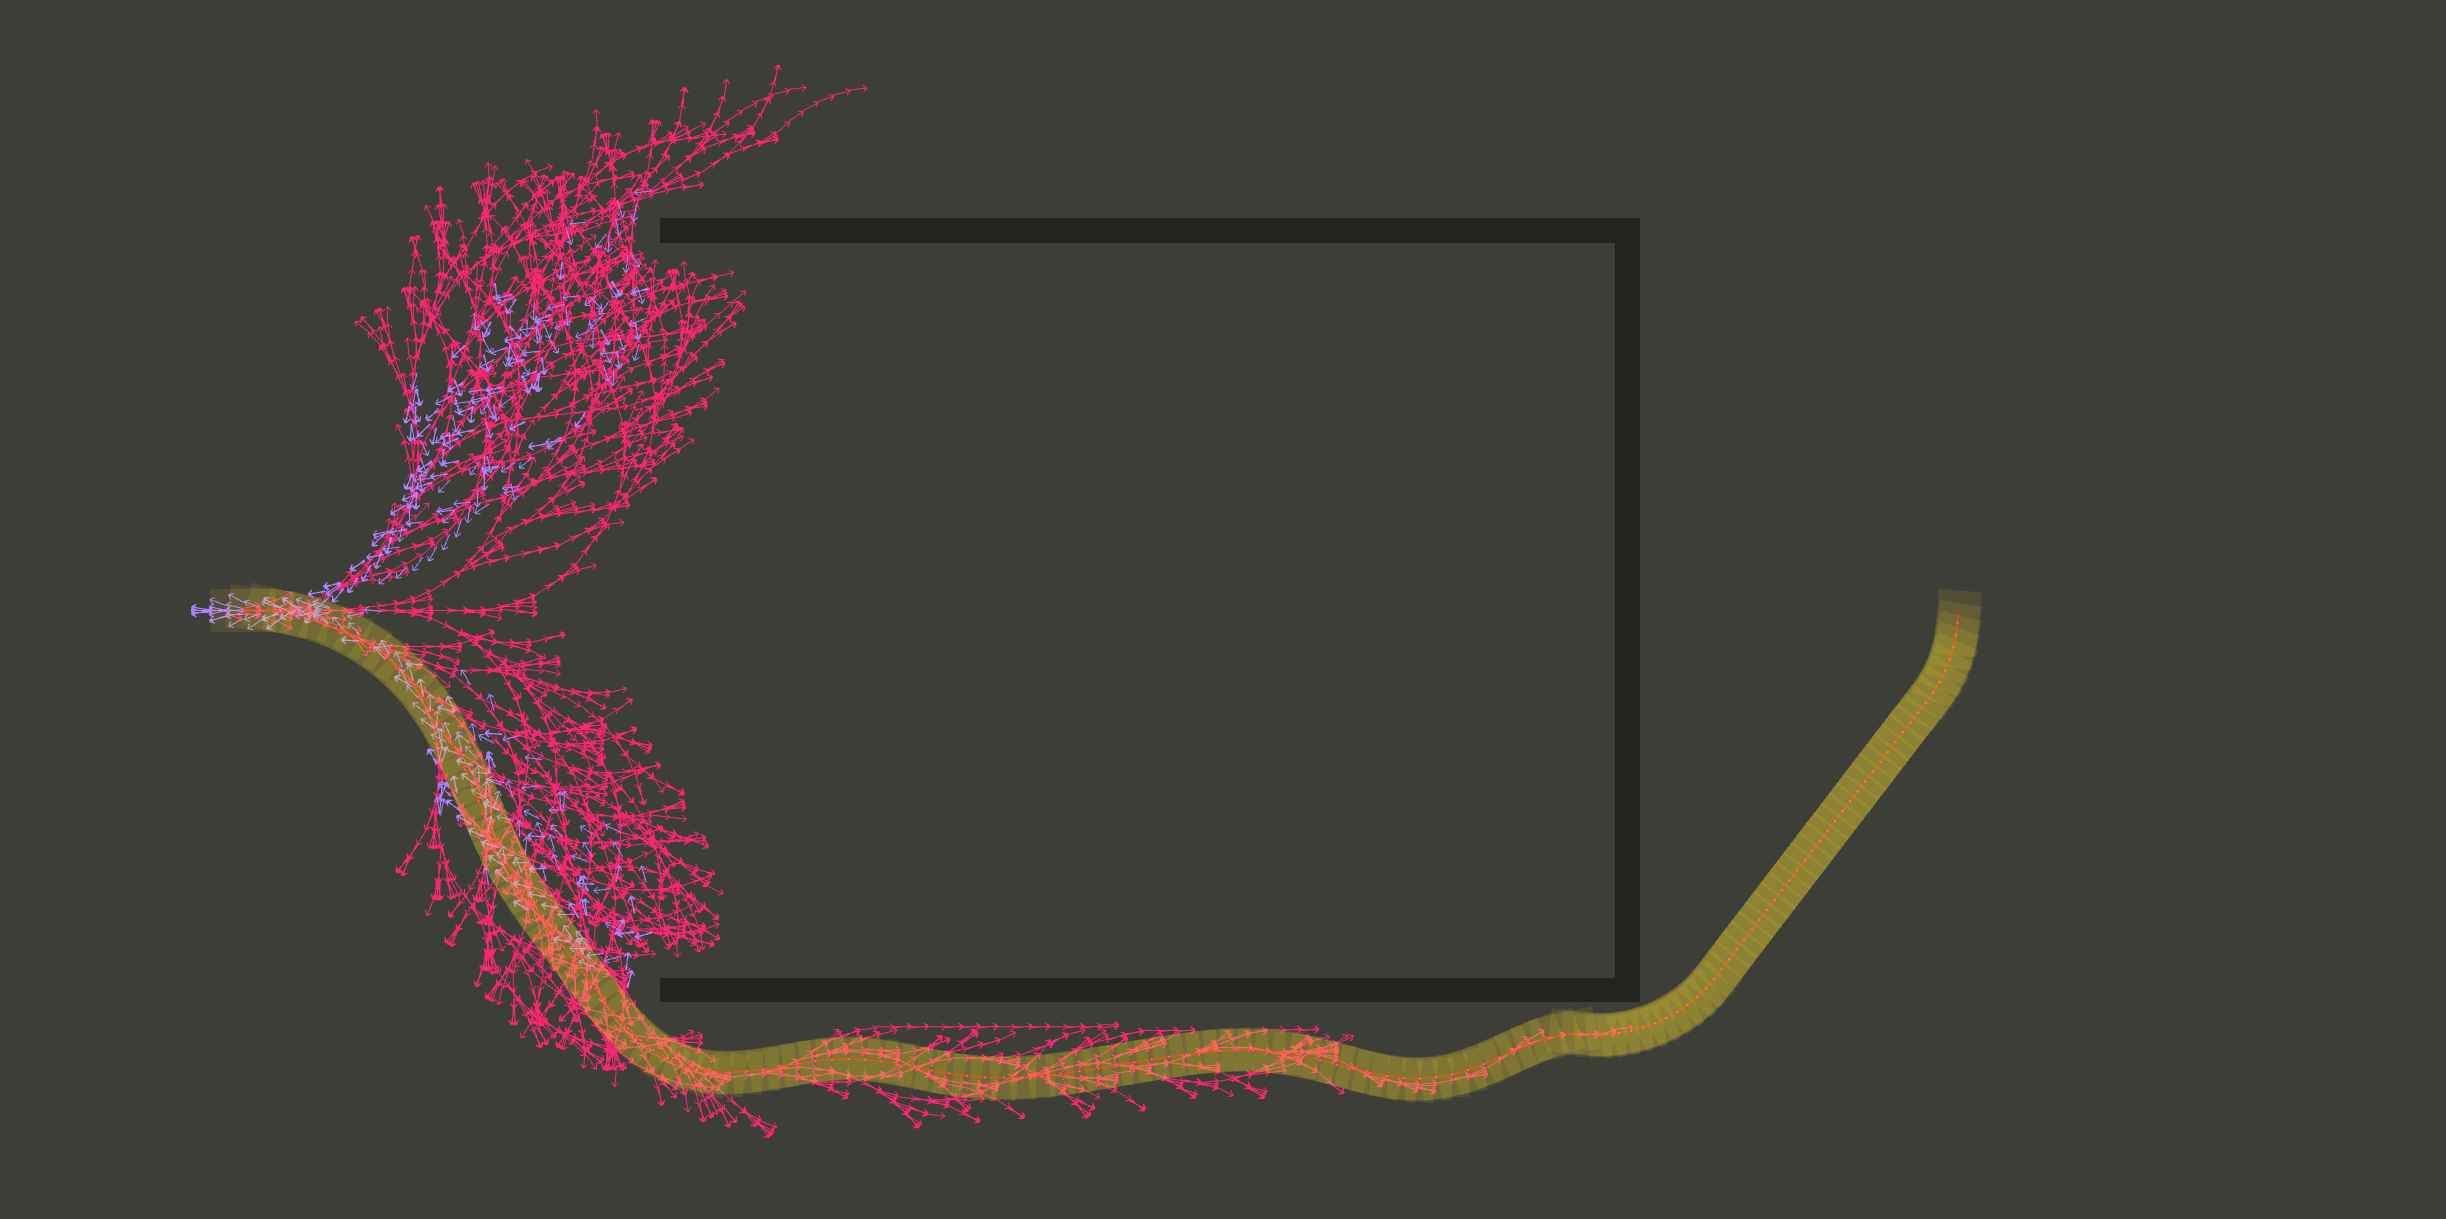
\includegraphics[width=\textwidth]{scenarioDeadEnd2dReedsShepp.png}
%        \caption{2D A* \& Dubins, 7829 vertices, length 91.5844\,m}
%        \label{fig:scenarioDeadEnd2dReedsShepp}
%    \end{subfigure}
    \caption{The dead end scenario}
    \label{fig:scenarioDeadEnd}
\end{figure}

\subsection{Additional Tests}

\begin{figure}[h]
    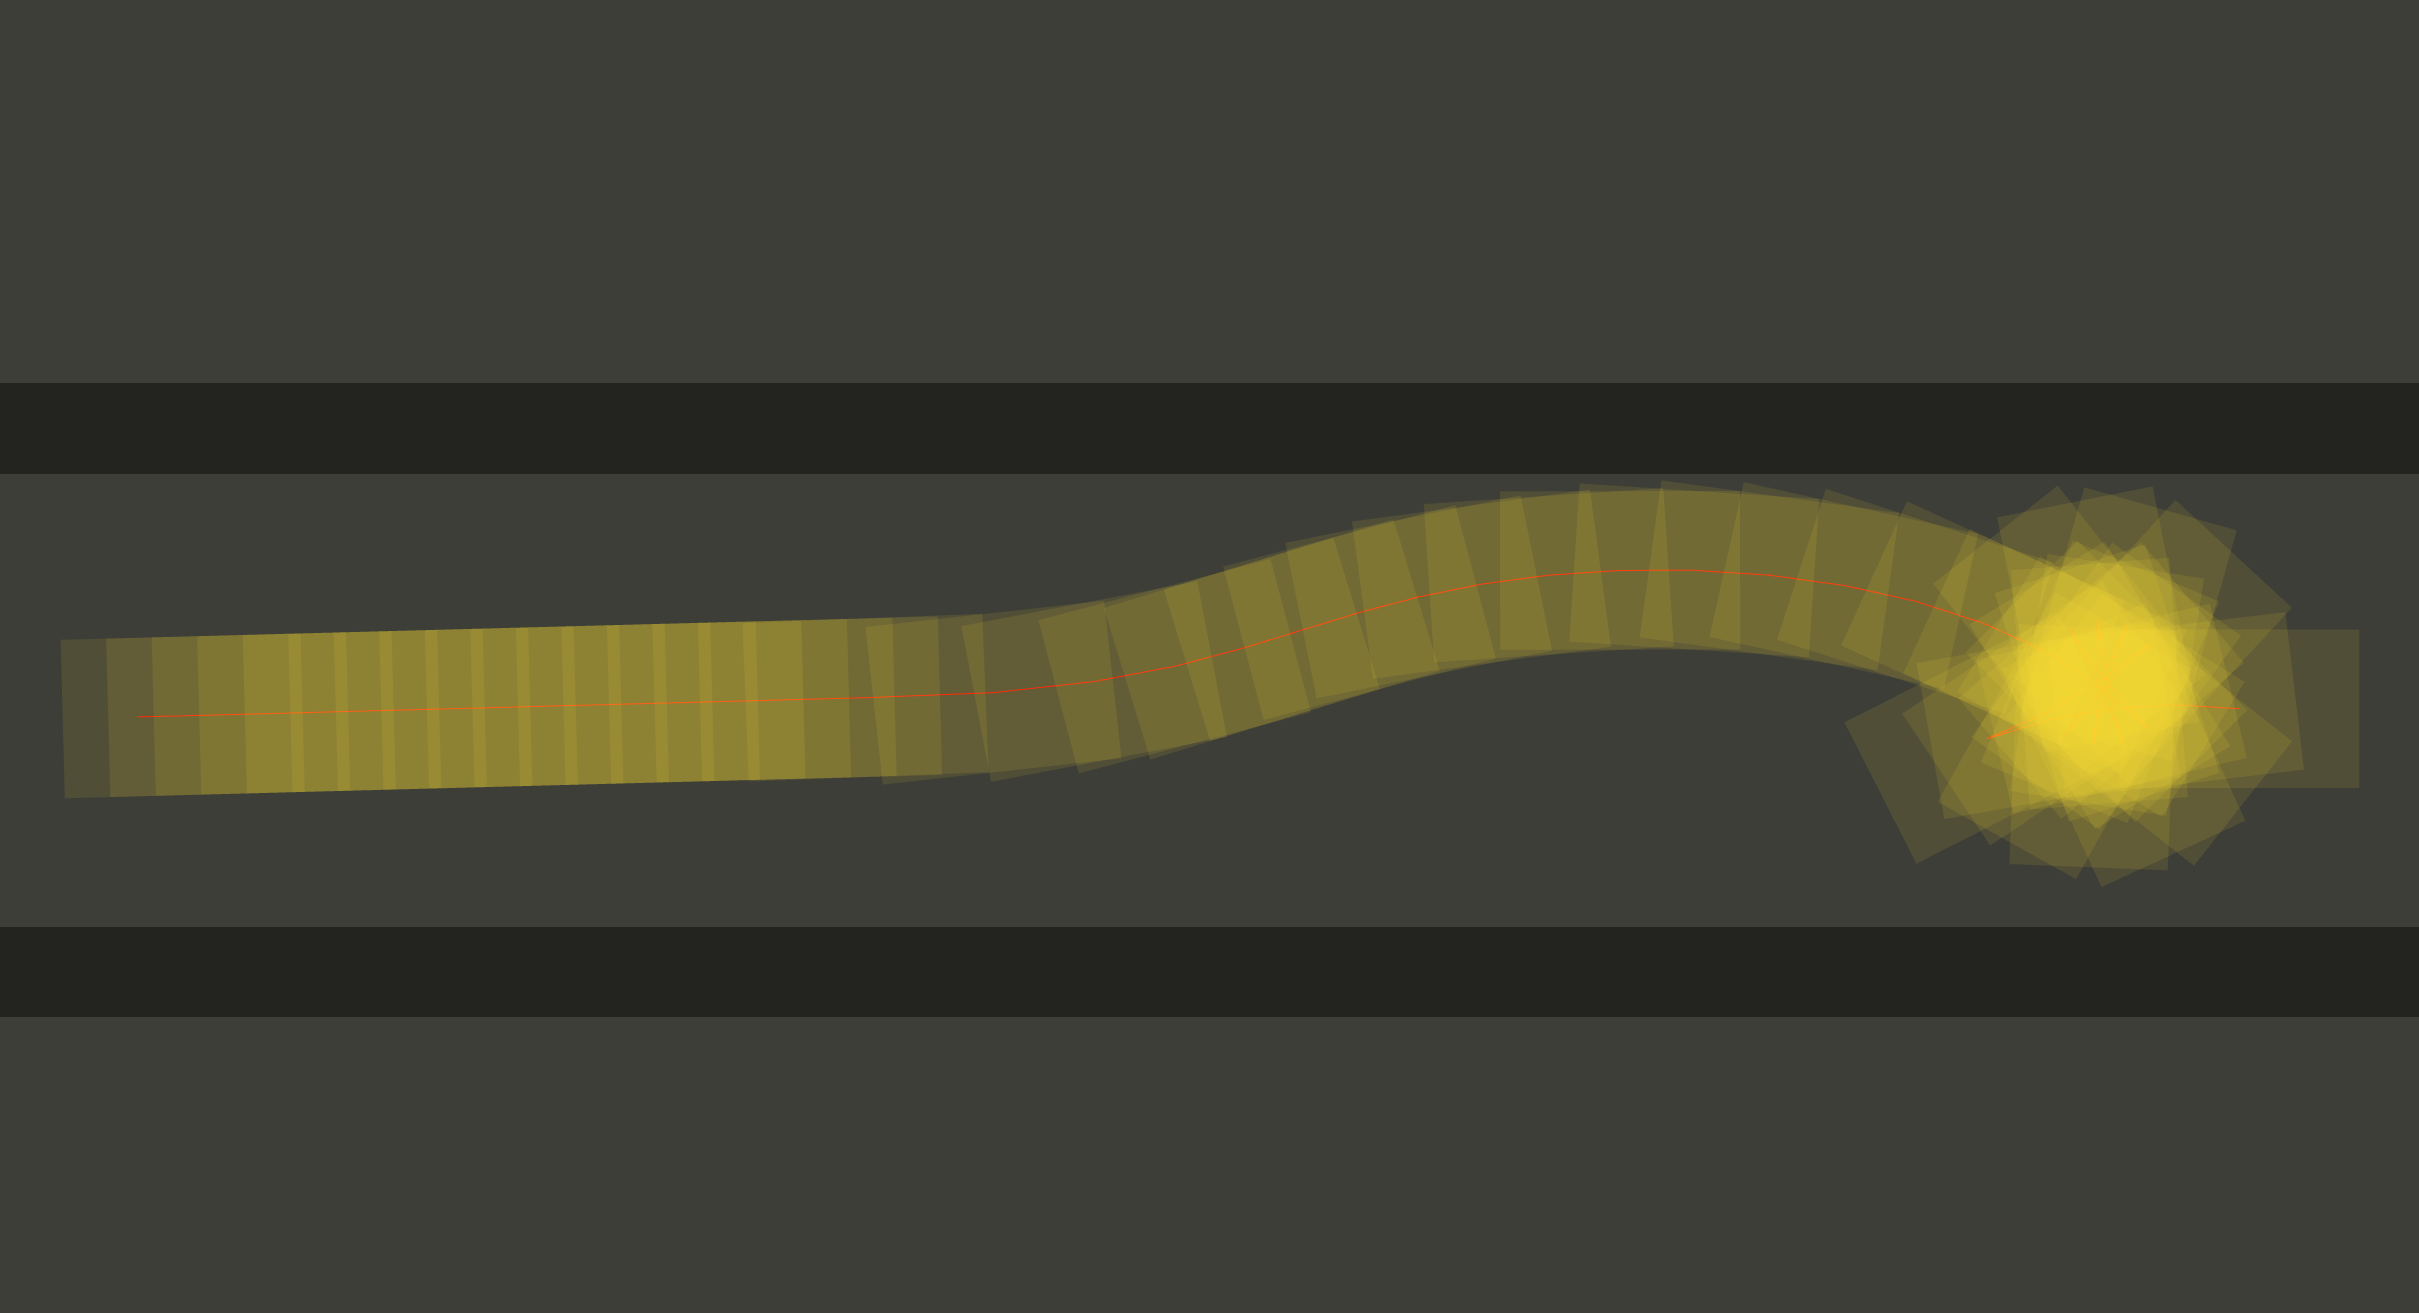
\includegraphics[width=\textwidth]{scenarioTurningSpot.png}
    \caption{Turning on the spot for change of directions}
    \label{fig:scenarioTurningSpot}
\end{figure}

\begin{figure}[h]
    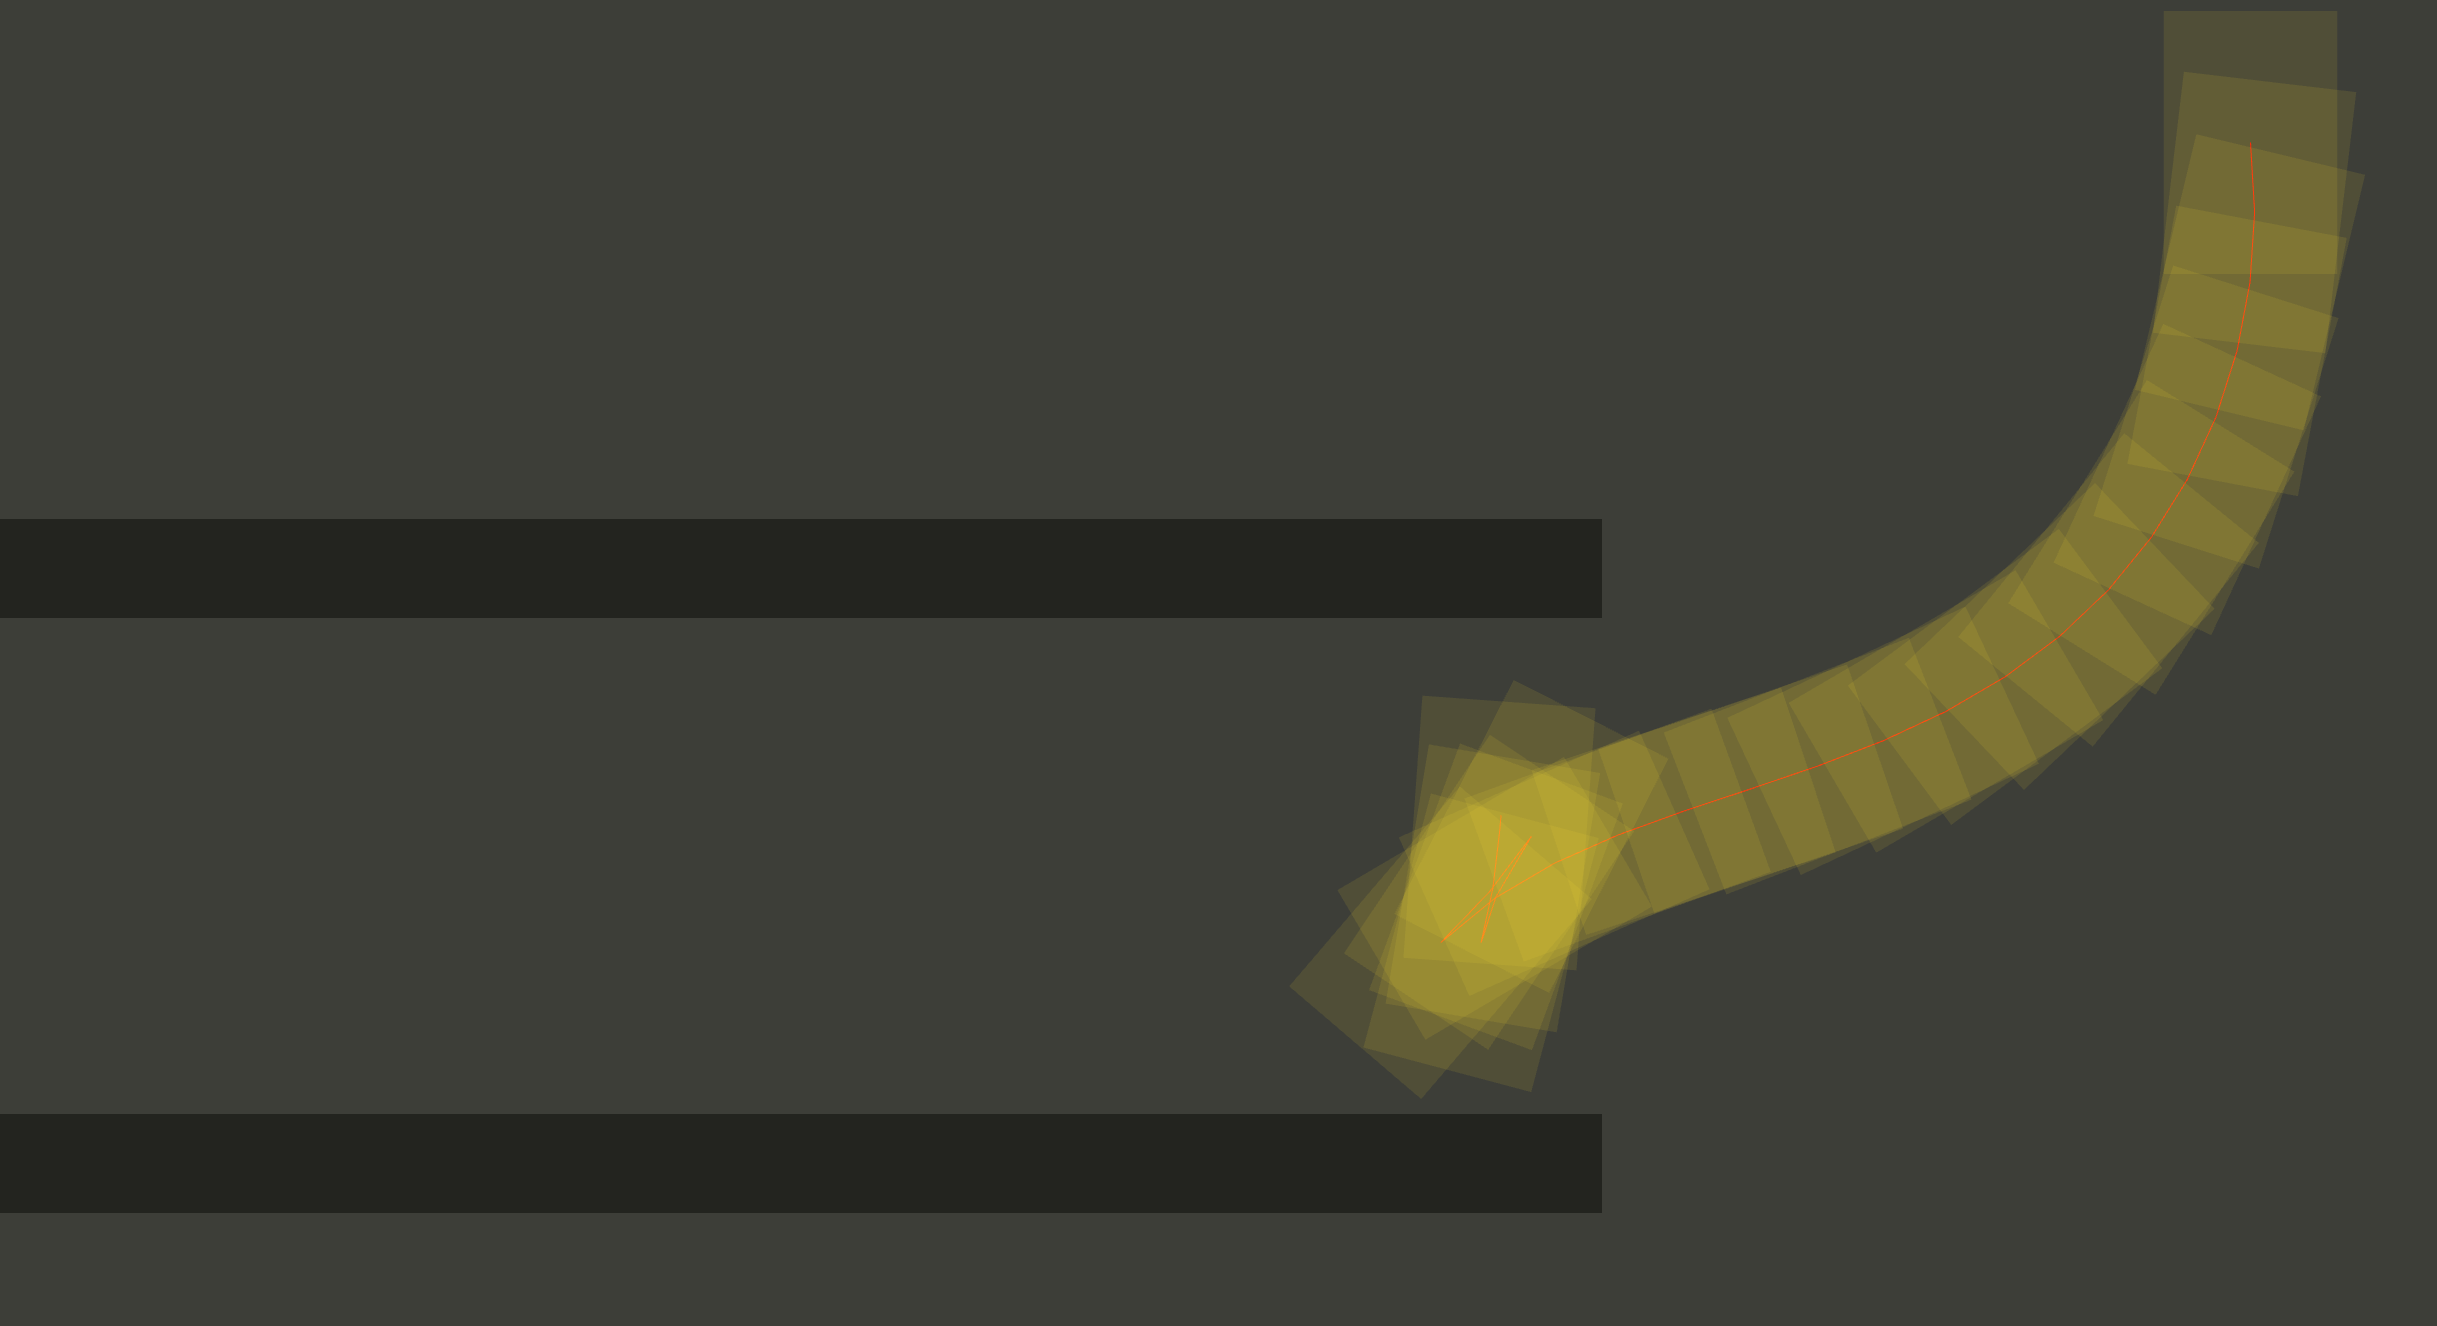
\includegraphics[width=\textwidth]{scenarioParallelParking.png}
    \caption{Parallel parking the car}
    \label{fig:scenarioParallelParking}
\end{figure}

%\begin{figure}[h]
%    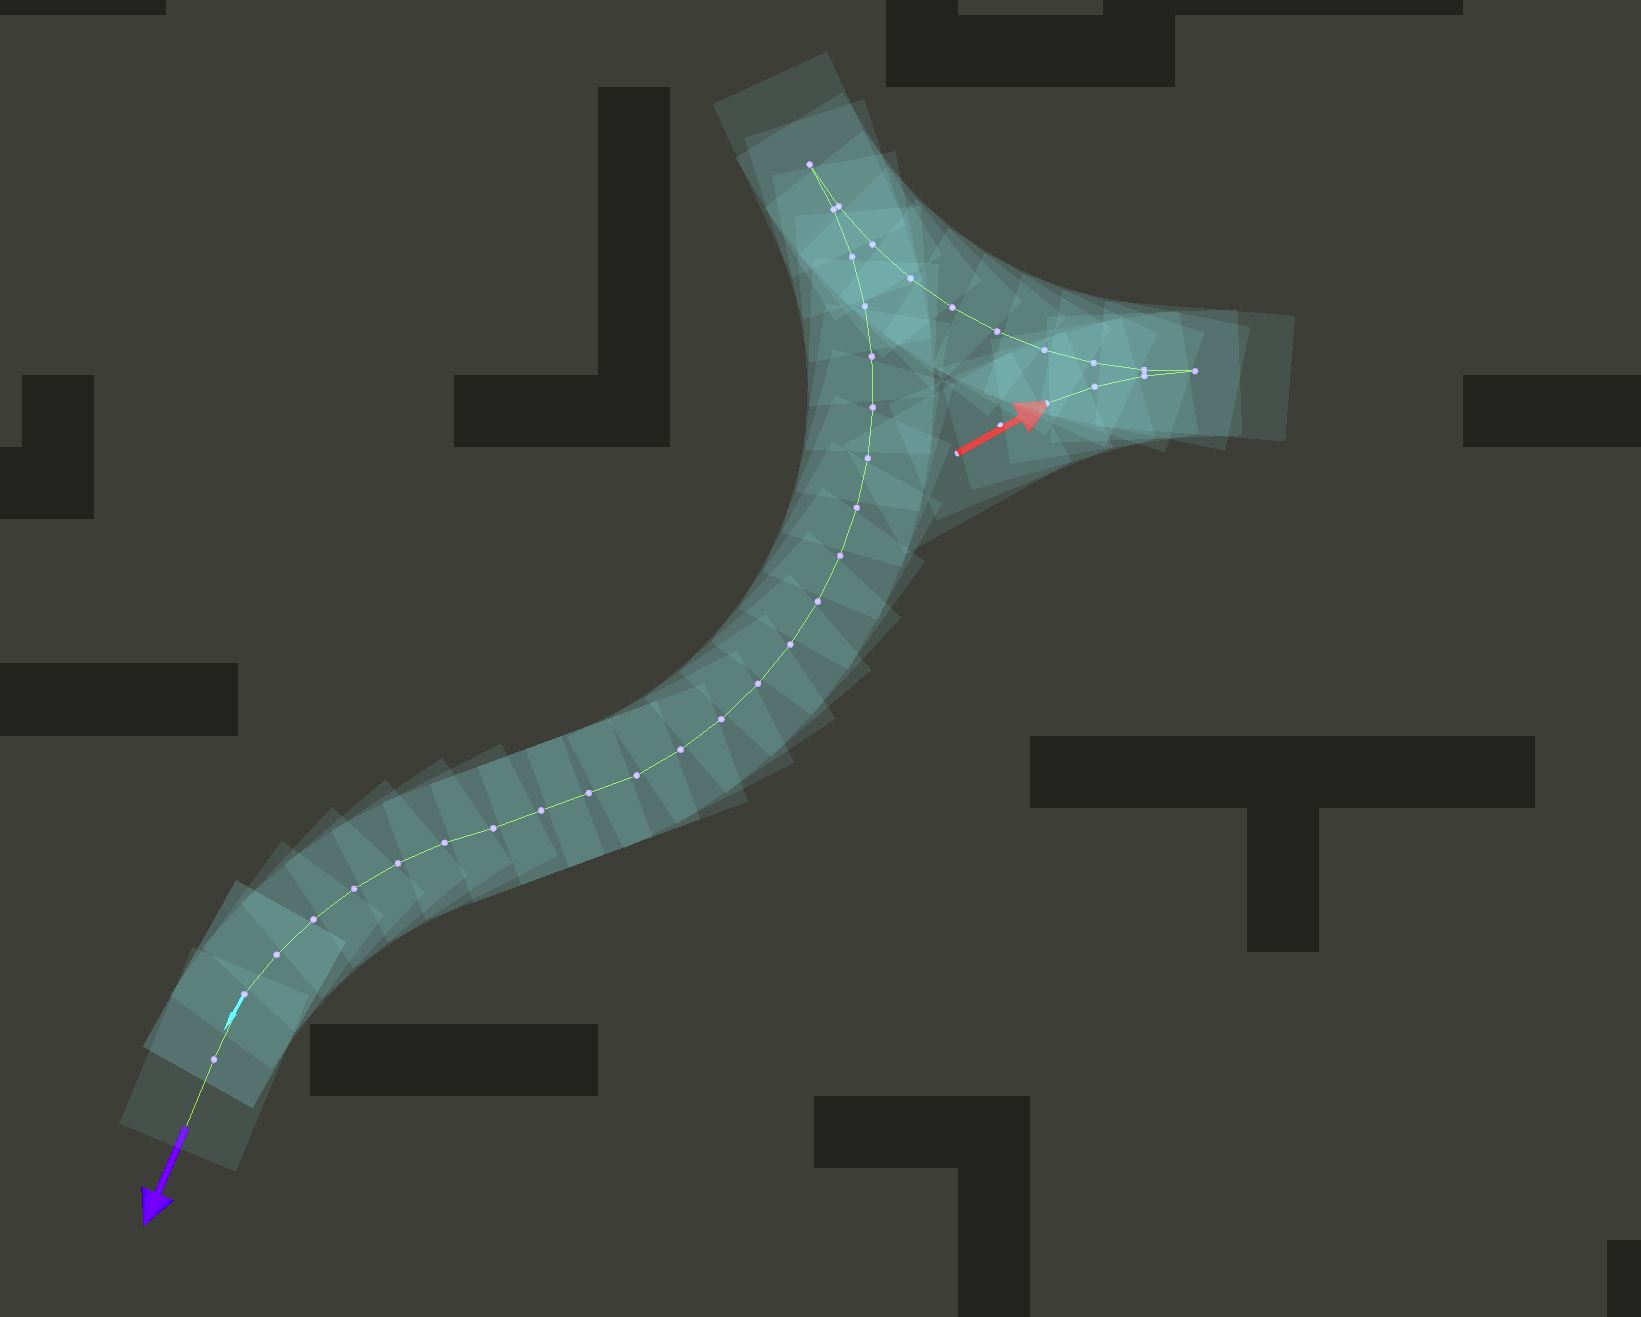
\includegraphics[width=\textwidth]{threePointTurn.png}
%    \caption{Three point turn for change of directions}
%    \label{fig:threePointTurn}
%\end{figure}
%
%\begin{figure}[h]
%    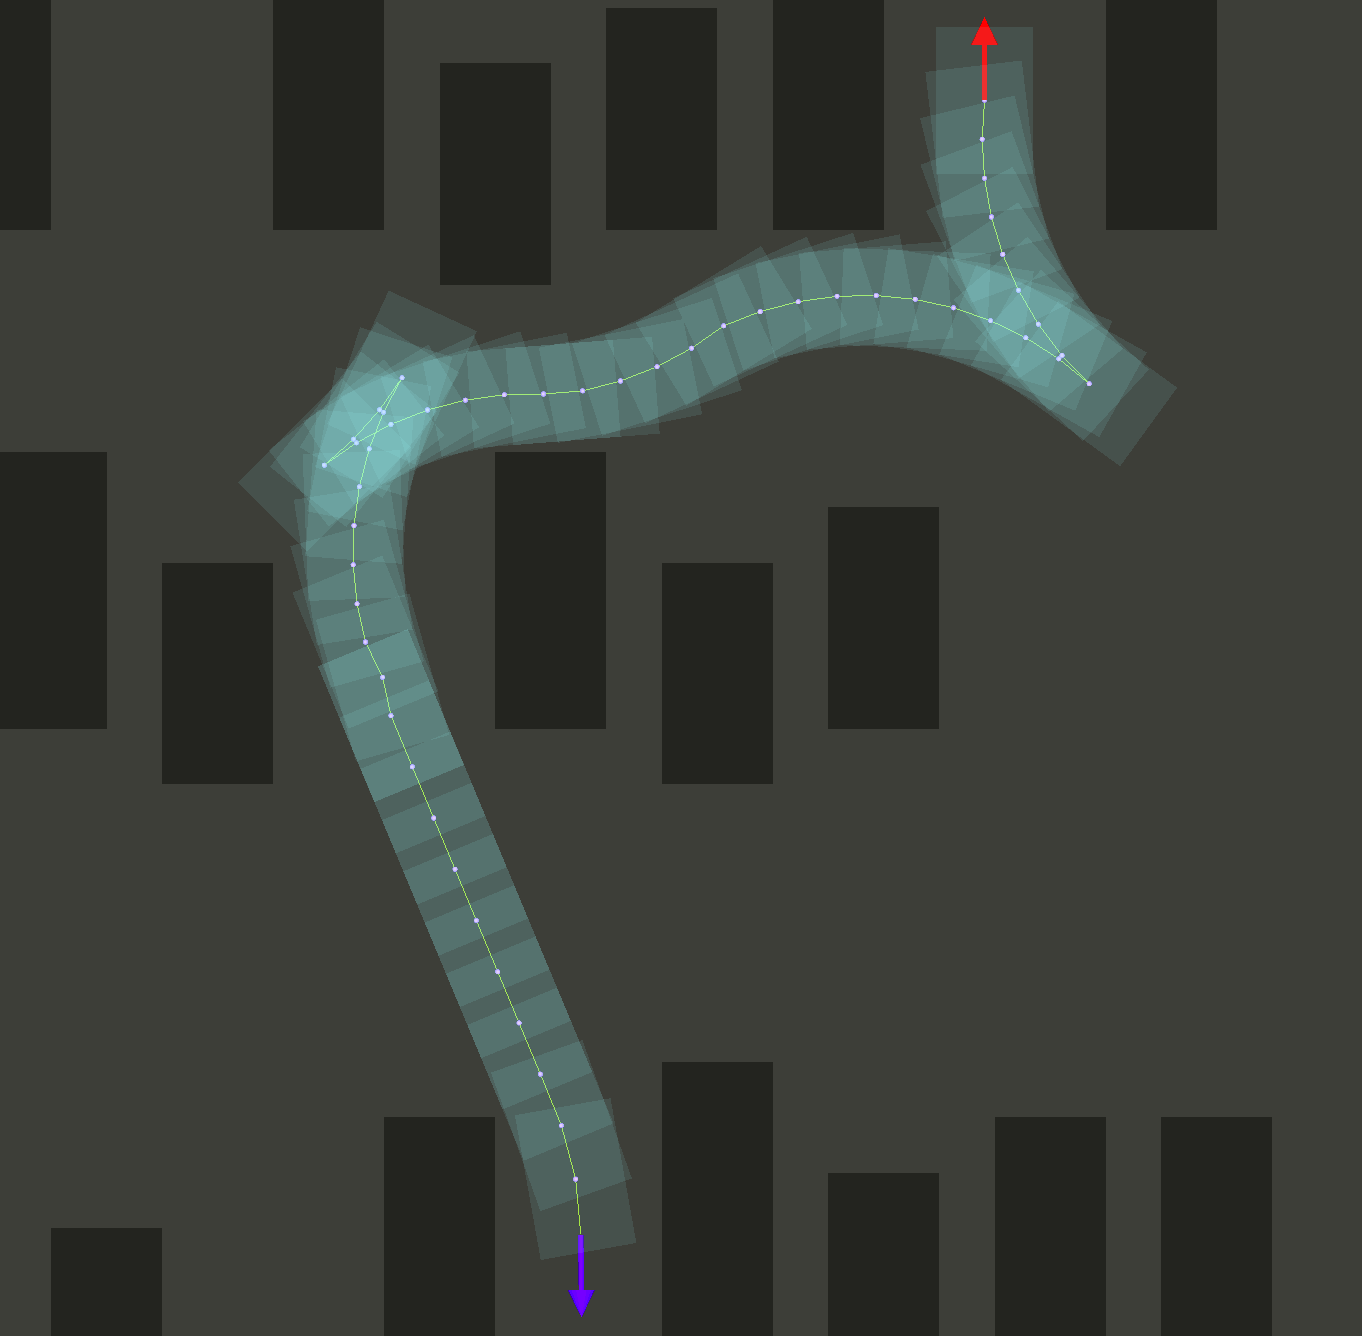
\includegraphics[width=\textwidth]{parking.png}
%    \caption{Change of parking spot in a parking lot}
%    \label{fig:parking}
%\end{figure}

\section{Real-world Results}